\documentclass[11pt,a4paper]{article}

\usepackage{amsmath,amssymb,bm}
\usepackage{amsthm}
\usepackage{booktabs}
\usepackage{array}
\usepackage{graphicx}
\graphicspath{{figures/}}
\usepackage[margin=1in]{geometry}
\usepackage[expansion=false]{microtype}
\usepackage{enumitem}
\emergencystretch=1.5em
\usepackage{xcolor}
\usepackage[numbers,sort&compress]{natbib}
\setlength{\bibsep}{0.5pt}
\renewcommand{\bibfont}{\footnotesize}
\usepackage[colorlinks=true,linkcolor=blue!60!black,citecolor=blue!60!black]{hyperref}

\newcommand{\TAN}{\textsc{Tan}}
\newcommand{\WTA}{\textsc{Wta}}
\newcommand{\eg}{\emph{e.g.}}
\newcommand{\ie}{\emph{i.e.}}
\newcommand{\cf}{\emph{cf.}}
\newcommand{\PassFailInconclusive}[1]{\textsc{pass}/\textsc{fail}/\textsc{inconclusive}}

\newtheorem{theorem}{Theorem}[section]
\newtheorem{lemma}{Lemma}[section]
\newtheorem{proposition}{Proposition}[section]
\newtheorem{corollary}{Corollary}[section]
\theoremstyle{remark}
\newtheorem*{remark}{Remark}

\title{\bf The Minimal Architectural Ladder for Relational Computation:\\[0.5ex]
From Temporal Saliency to Binding and Composition\\in a Dynamical Neuron Model}
\author{Li Zexu\\
School of Physics and Astronomy, University of Leeds\\
\texttt{correspondence: [correspondence email pending submission]}}
\date{Final Revised Manuscript (September 2026)}

\begin{document}
\maketitle

\begin{abstract}
Modern computational neuroscience and deep learning routinely conflate five
distinct computational primitives---memory, saliency weighting, content
routing, semantic binding, and composition---and infer the emergence of the
higher ones from increases in dynamical complexity alone. This paper replaces
that inference with a constructive question: given a fixed dynamical substrate,
which minimal organizational degree of freedom must be added to ascend from one
primitive to the next? We answer the question inside a single dynamical unit,
the Temporal Attention Neuron (\TAN), whose scalar-input, scalar-gate
surprise-weighted kernel was previously frozen (TAN-I) as a system that is
historically dependent, geometrically responsive, and yet provably incapable of
query-conditioned routing. Proceeding one degree of freedom at a time and
auditing every step with counterfactual suites and negative-control chains, we
establish six principal results. (i) Excitatory--inhibitory opponent topology suffices
for nonmonotonic selective tuning but not for routing
($\text{Competition}\not\Rightarrow\text{Routing}$; six layouts,
$\mathrm{FlipRate}\equiv0.000$). (ii) Two-dimensional vector query--key
interaction unlocks routing capacity with an exact geometric law,
$\mathrm{FlipRate}_{\mathrm{CF}}(\theta)=\theta/\pi$ (132/132 Monte Carlo
conditions), and realizes counterfactual winner flips in the running neuron
(fixed history, query $3\to4$: margin $+0.2587\to-0.1559$; ensemble
$0.4425$ vs.\ benchmark $0.4445$). (iii) Key--value decoupling yields soft
binding, and the winner-take-all limit ($\gamma\to\infty$) yields exact,
lossless delivery while leaving routing statistics unchanged---the first
orthogonal axis: \emph{routing selectivity $\perp$ readout discreteness}.
(iv) A single head cannot simultaneously deliver two distinct bound operands to downstream algebra ($\text{Binding}\not\Rightarrow
\text{Composition}$); while a single head can evaluate symmetric pooling functions, two parallel channels plus one minimal two-input
algebraic node are required to achieve zero composition error conditioned on correct binding,
with all unconditional error attributable to upstream routing---the second
orthogonal axis: \emph{binding fidelity $\perp$ combiner error}.
(v) Auditing address identifiability in multi-candidate retrieval ($N=3$, 60,000 trials, 420,000 model evaluations) proves that scalar dot-product kernels mathematically cannot address intermediate keys ($0/6{,}705$ hits, $0.00\%$), whereas a one-dimensional metric distance kernel achieves $100.00\%$ routing identical to two-dimensional vector rotation under hard selection, proving that metric compatibility rather than multidimensional rotation is the true mathematical boundary of content addressing.
(vi) A pre-registered confirmatory audit of continuous dynamical carriers and discrete spiking readouts (Phase~P1-B, 96,000 episodes, 192,000 queries) certifies that subthreshold inputs undergo analytical state collisions erasing history, baseline dynamical carriers fail prerequisite delivery floors ($2.75\%$--$2.90\%$ joint accuracy), rendering memory comparisons floor-limited with memory redundancy unestablished, and single-unit spiking readouts exhibit severe transmission breakdown ($E_{\text{comp}} \in [2.21, 2.57]$, $82\%$ abstention), certifying model-specific carrier insufficiency and point-process transmission limits while deferring internal composition dynamics. The result is
a unified, stepwise mechanistic ladder of relational computation and an
explicit map of the walls that separate its rungs.
\end{abstract}

% ==========================================================================
% Paper 2 — Section 1: Introduction. The Conflation Problem and the
% Architectural Stance.
% All quantitative statements in this section are forward pointers to the
% frozen archives; the numbers themselves are stated and sourced in the
% sections that own them (§3–§8).
% ==========================================================================
\section{Introduction: The Conflation Problem and the Architectural Stance}
\label{sec:intro}

\subsection{The conflation problem}
\label{sec:conflation}

A striking feature of the modern literature on attention, memory, and
relational computation is that its central vocabulary is used
interchangeably across levels that are causally distinct. A network that is
``attentive'' is described as routing information; a unit whose output is a
weighted mixture of stored items is described as binding them; a system that
can retrieve two stored values is described as composing them. Underneath
this vocabulary sits a chain of five primitives---\emph{memory},
\emph{saliency weighting}, \emph{content routing}, \emph{semantic binding},
and \emph{composition}---each of which imposes its own, strictly stronger,
requirement on the substrate that realizes it. When these are conflated, the
classic inferential error follows: observing the \emph{lower} primitive,
together with rich nonlinear dynamics, is taken as evidence for the
\emph{higher} one. Four examples of the conflation recur in our own field of
view: (a) \emph{history dependence $\Rightarrow$ attention routing}---a
non-Markovian hidden state does not imply that a query can reorder candidate
preferences; (b) \emph{attention weighting $\Rightarrow$ semantic
binding}---a softmax mixture over stored items delivers a convex combination,
not a bound symbol; (c) \emph{sharpening $\Rightarrow$ selection}---any finite
temperature keeps every candidate weight strictly positive, so sharpening
approaches, but never achieves, discrete delivery; and (d) \emph{retrieval
$\Rightarrow$ composition}---delivering two values into a pair is not the
same as applying a deterministic algebraic relation to them.

This is not merely a semantic complaint. End-to-end training of monolithic
networks makes the conflation unfalsifiable in practice: every stage of a
black-box system co-varies under optimization, so post hoc attribution of a
capability to a mechanism is, in general, impossible \citep{fodor1988,
lake2017,lake2018}. The binding problem of classical neuroscience is the
canonical instance: synchrony, assembly formation, and indexing have all been
proposed as binding mechanisms \citep{von1995,singer1999}, yet a demonstration
that a candidate mechanism \emph{binds}, as opposed to merely re-weights, is
rarely separated from the demonstration that it \emph{routes}. What the field
lacks is not more powerful models but a \emph{boundary map}: for each rung of
the primitive ladder, the minimal structural condition under which the
primitive becomes observable in a dynamical substrate, and a falsifiable test
that separates it from the rungs below.

\subsection{Thesis and methodological stance}
\label{sec:stance}

The thesis of this paper is architectural rather than dynamical:

\begin{quote}
\emph{Computational capability is constrained not only by nonlinear
dynamics, but by the organizational degrees of freedom available to the
dynamics.}
\end{quote}

More dynamics---richer nonlinearities, larger state spaces, longer memory
windows---does not, by itself, produce new computational primitives. It
provides a richer \emph{stage}; the primitives are provided by the
\emph{topological organization} of the computation. To make the thesis
testable we adopt two disciplines that run through the entire study.

\emph{Radical minimalism.} The substrate is a single dynamical unit---the
Temporal Attention Neuron (\TAN) of the frozen TAN-I archive---a leaky,
spiking neuron whose input current is a surprise-gated, temporally attended
mixture of its recent inputs (§2.3). It is deliberately the smallest system
in which the conflation (a)--(d) can be exhibited, because every confound
that a larger network would introduce (depth, width, training, shared
substrates) is absent by construction.

\emph{The single-degree-of-freedom ladder.} Each step of the study changes
exactly one organizational degree of freedom and leaves the frozen dynamics,
window, gates, and readouts untouched (§2.4). After each step, the new
configuration is audited by counterfactual experiments---identical histories
with only the query changed---and by negative-control chains in which the
preceding rung of the ladder is shown to fail the same test (§2.5). A rung is
claimed only if the audit passes under the joint criteria, never from a
single scalar error.

We state the resulting scope preemptively. This paper does not propose a
network that beats any benchmark; it proposes a \emph{constraint map} for
dynamical computation. Its results are \emph{sufficiency} statements within
one explicitly frozen mechanism family, not necessity statements about
brains or about all possible machines; and negative results are reported
with the same status as positive ones. Readers expecting accuracy tables
will find boundary tables instead; that is the intended product.

\subsection{Why a single neuron is the right test bed}
\label{sec:testbed}

The TAN-I programme established the bottom two rungs of the ladder inside
this substrate, and---decisively---located the first wall above them. In
brief (full numbers and protocols in §3--§5): the scalar TAN is
historically dependent and its membrane potential is not a sufficient
Markov state (Phase 1: $N=160{,}000$ collision experiments; state
insufficiency lemma), so \emph{memory} is realized. Its surprise-gated
attention reshapes the event-locked response geometry of the system
(Phase 2: effective rank $d_D\approx2.089$ under attention versus
$\approx1.484$ without), so \emph{saliency weighting} is realized and is
geometrically effective. Yet two negative probes froze the boundary:
a temporal distractor task showed no robustness premium attributable to
attention, and a formal binding audit---the query-conditioned
identifiability audit, archived as \textsc{terminated /
audit\_failed}---recorded a counterfactual argmax flip rate of exactly
$0.000$: the scalar kernel $E_{t,i}=\beta W_qW_k\,S_t\,x_i$ can rescale
candidate logits but can never reorder them, because its ``query'' is the
non-negative scalar surprise cone $\mathcal{Q}_+=[0,\infty)$. Scalar
saliency, in other words, lies \emph{below} routing on the ladder, and the
gap is provable rather than empirical (the order-conservation theorem,
§5). The TAN therefore leaves us exactly where a mechanism study should
start: at a wall, with a clean statement of which side each frozen result
belongs to.

\subsection{Contributions and roadmap}
\label{sec:contrib}

The present paper (TAN-II, sprints 4.1--4.3-A) ascends the ladder one degree
of freedom at a time and reports the following results.

\begin{enumerate}
\item \textbf{Competition without routing (§4).} Adding
excitatory--inhibitory opponent topology to the frozen neuron produces
nonmonotonic selective tuning by analytic construction---the E-I
nonmonotonicity theorem---and the static opponent control shows the peak
exists with \emph{no} attention at all ($x^*=1.00$, $h_E=0.200$), severing
the attribution of local tuning to attention. Attention is thereby redefined
as dynamic gain and operating-range modulation. Across six layouts the
counterfactual flip rate remains exactly $0.000$:
$\text{Competition}\not\Rightarrow\text{Routing}$.
\item \textbf{The geometric boundary of routing (§5).} Two-dimensional
vector query--key interaction unlocks routing capacity with an exact law,
$\mathrm{FlipRate}_{\mathrm{CF}}(\theta)=\theta/\pi$ (132/132 Monte Carlo
conditions; winner measures $1/2$; the winner-variation statistic $F_d=1/2$
constant across $d\in\{2,3,4,8\}$ as a negative control). In the running
neuron, changing only the query from $3$ to $4$ on a fixed history flips the
attention winner with margins $+0.2587\to-0.1559$ (closed-form crossing
$Q^*=3.7071$; ensemble flip rate $0.4425$ vs.\ quadrature benchmark
$0.4445$), and key normalization is shown to be a mechanistic enabler, not a
cosmetic control.
\item \textbf{From routing to binding, and to exactness (§6--§7).}
Key--value decoupling yields soft binding whose value-transfer is
winner-aligned and provably pairing-sensitive ($T_{\mathrm{swap}}=-T$ to
$10^{-12}$), with a softness distance $D\approx1.7$--$1.8$ inherited from
softmax convexity. The winner-take-all limit $\gamma\to\infty$ achieves
exact, lossless delivery while the routing statistics
($\mathrm{FlipRate}\approx0.4445$) remain exactly flat across the entire
sharpening ladder---the first orthogonal axis:
\emph{routing selectivity $\perp$ readout discreteness}.
\item \textbf{From binding to composition (§8).} A single head is a
bottleneck: it delivers one scalar symbol per instant and cannot simultaneously
deliver two distinct bound operands to general downstream algebra, so binding
alone cannot compose general arithmetic ($\text{Binding}\not\Rightarrow\text{Composition}$;
the three-error joint audit catches the $V_A=0$ accidental-zero trap). Two parallel channels
plus one minimal two-input algebraic node achieve composition with
\emph{zero} error conditioned on correct binding, over $3\times10^4$
Monte Carlo histories ($E[E_{\mathrm{comp}}|\text{both-routed}]\equiv0$,
$\max=0$), while all unconditional error is attributable to upstream
routing---the second orthogonal axis:
\emph{binding fidelity $\perp$ combiner error}.
\end{enumerate}

These results assemble into the unified mechanistic ladder of §9 and the
graded claim ledger of §10. The through-line of the paper is that each rung
corresponds to one \emph{named} organizational degree of freedom---opponent
topology, vector interaction, key--value decoupling, discrete selection,
parallel channels, and an algebraic node---and that each rung can be
assigned a falsifiable boundary test. More dynamics did not have to be
added at any step; organization did.

The remainder of the paper is organized as follows. §2 gives the formal
framework: axiomatic definitions of the five primitives, the frozen
baseline model, the catalog of extension operators, and the audit
methodology. §3 records the state and geometry baseline inherited from
TAN-I. §4–§8 present the five rungs and their audits in ladder order.
§9 assembles the master table, discusses the biological reading of each
degree of freedom (opponent microcircuits, oscillatory phase, dendritic
subunits, axonal threshold integration), and states the general discussion.
§10 closes with the claim ledger and the reproducibility statement.

% ==========================================================================
% Paper 2 — Section 2: Formal Framework. Five Primitives, the Frozen
% Baseline, the Extension-Operator Catalog, and the Audit Methodology.
% ==========================================================================
\section{Formal Framework: Five Primitives and the Frozen Baseline}
\label{sec:framework}

This section fixes the definitions that the remainder of the paper uses
without further negotiation: the five computational primitives (§2.2), the
frozen dynamical baseline they are tested against (§2.3), the catalog of
single-degree-of-freedom extensions that ascend the ladder (§2.4), and the
audit methodology by which every rung is either established or rejected
(§2.5). All quantitative constants in this section are taken verbatim from
the frozen archives (TAN-I and TAN-II sprints 4.1--4.3-A); none are free.

\subsection{Notation and conventions}
\label{sec:notation}

Time is discrete, $t\in\mathbb{N}$. Inputs are scalar amplitudes
$x_t\in\mathbb{R}$; the temporal window is the ordered $W$-tuple
$X_t=(x_{t-W+1},\ldots,x_t)$ with zero padding at onset. We write
$[z]_+=\max(z,0)$ for rectification, $\Theta(\cdot)$ for the Heaviside
step, $\sigma(z)=1/(1+e^{-z})$ for the logistic function, and
$\operatorname{softmax}_i(\bm e)$ for the normalized exponential map.
In Sprint~4.2-B/C/D the standard max-stabilized form
$\alpha_i=\exp(e_i-\max_k e_k)/\sum_j\exp(e_j-\max_k e_k)$ is evaluated
directly without offset ($\sum_i\alpha_i=1.0$ exactly), whereas the baseline
model implementation (\texttt{tan.py}) added a numerical stabilizer
$\delta=10^{-9}$ to the denominator. Alternative mappings that induce exact
sparsity without infinite gain, such as sparsemax \citep{martins2016}, are
discussed as theoretical comparisons. Candidate sets are always
finite. A \emph{counterfactual pair} is a pair of experimental conditions
that share the identical history content and differ only in the query; a
\emph{negative-control chain} is a sequence of models $M_0,M_1,M_2$ in which
each model adds exactly one organizational degree of freedom and the
preceding model is required to fail the criterion that the following model
is required to pass.

\subsection{The five primitives, operationally defined}
\label{sec:primitives}

The paper's object is the chain
$\text{Memory}\to\text{Saliency}\to\text{Routing}\to\text{Binding}\to
\text{Composition}$. Each primitive is defined by an operational criterion
that a frozen experiment can pass or fail; the criteria are the ones
actually used in the audits of §4--§8. The chain is constructive: in the
mechanism family tested here, each later primitive presupposes the earlier
ones, while the central negative results of this paper show that none of
the reverse implications holds.

\begin{description}[style=nextline,leftmargin=2em]
\item[P1 --- Memory.] \emph{Definition.} A system has memory relative to a candidate
state variable if its future evolution depends causally on aspects of the input history
that are not recoverable from that candidate state. \emph{Criterion} (TAN-I Phase 1, §3):
the one-dimensional scalar membrane potential $h_t$ is not state-sufficient; the projection
$(h_t,X_t)\mapsto h_t$ is not lumpable. Two histories with equal membrane potentials but
different window contexts produce different downstream trajectories (quantified by pairwise
separation $K$ and post-reset divergence). This demonstrates state non-sufficiency of scalar $h_t$;
it does not imply that the complete Markovian state $(h_t, X_t)$ violates Markovianity, nor
that Markovian dynamics imply state-space contraction.
\item[P2 --- Saliency weighting.] \emph{Definition.} A system performs saliency weighting
if its readout over a fixed candidate set preserves relative ranking across all active query
levels. Under standard continuous softmax (whose support is everywhere strictly positive,
in contrast to sparse activation functions such as sparsemax \citep{martins2016}), the defining
signature of scalar modulation is not support-set invariance, but rather \emph{ranking invariance}:
for all $S>0$, the induced ordering of attention weights $\alpha(Q)$ is strictly invariant,
and $\operatorname{argmax}_i\alpha_i(Q)$ is independent of query content. \emph{Criterion:}
Rank-1 kernel factorizability $E(Q, K) = q(Q)\cdot k(K)$ is a sufficient condition ensuring
that positive scalar query modulation acts purely as a monotonic gain on logit differences,
\item[P3 --- Content routing.] \emph{Definition.} A system routes if there
exist queries $Q_A,Q_B$ and a fixed history such that
$\operatorname{argmax}_i R(Q_A,K_i)\neq\operatorname{argmax}_i R(Q_B,K_i)$.
In multi-candidate memory ($N\ge3$), true content addressing requires selective
identifiability: for every candidate key $K_t$, there exists a query making $K_t$ the
unique maximum. While separable dot-product kernels $E(Q, K) = Q K$ in $\mathbb{R}$
can at most invert global order between the extreme elements without addressing intermediate keys
(Proposition~\ref{prop:scalar_impossible}), metric compatibility kernels $E(Q, K) = -(Q-K)^2$
achieve universal addressability even in $d=1$ (Proposition~\ref{prop:metric_suff}).
\emph{Criterion:} the counterfactual flip rate
$\mathrm{FlipRate}_{\mathrm{CF}}$ is nonzero on a fixed-history ensemble;
capacity (the geometric existence of flips) and realization (the running
model actually flipping) are reported separately (\S\ref{sec:routing}).
\item[P4 --- Semantic binding.] \emph{Definition.} A system binds if
role/address (key) and content entity (value) are decoupled and the output
transmits the value of the \emph{selected} key, following the
(key,value) association rather than key identity, position, or amplitude.
\emph{Criterion:} the value-swap counterfactual is antisymmetric,
$T_{\mathrm{swap}}=-T$ exactly, and the softness distance
$D=|C-v_{\mathrm{winner}}|$ is measured; hard binding is the limit $D=0$.
\item[P5 --- Composition.] \emph{Definition.} A system composes if it applies
a deterministic algebraic relation $f$ to at least two independently
retrieved bound values, $y=f(V_A,V_B)$. \emph{Criterion:} the three-error
joint audit of §2.5 (binding errors and composition error simultaneously
$\approx0$) together with the counterfactual suite of §8 (query swap, value
swap, key swap, channel-output swap, the zero-value trap, and the
binding-preserving, binding-breaking, and relational controls); conditioned
on correct binding the composition error must be exactly zero (the
binding--combiner separation test).
\end{description}

\subsection{The frozen baseline: the scalar Temporal Attention Neuron}
\label{sec:baseline}

The substrate is the TAN-I Temporal Attention Neuron, frozen before this
study and never retrained or retuned here. Its computation chain is

\begin{align}
\mu_t &= \frac{1}{W}\sum_{k=0}^{W-1} x_{t-k}, \qquad
S_t=[x_t-\mu_t-\varepsilon]_+,
\label{eq:surprise}\\
E_{t,i}&=\beta\,W_q W_k\,S_t\,x_{t-i}, \qquad
\alpha_{t,i}=\frac{\exp(E_{t,i})}{\sum_j\exp(E_{t,j})+\delta},
\label{eq:kernel}\\
C_t&=\sum_i \alpha_{t,i}\,x_{t-i}, \qquad
A_t=\tanh(S_t)\,C_t,
\label{eq:context}\\
h_t&=\lambda\,h_{t-1}+A_t, \qquad
y_t=\Theta(h_t-\theta_{\mathrm{sp}}), \qquad
h_t\leftarrow 0\ \text{on spike}.
\label{eq:membrane}
\end{align}

Three properties of this chain carry the whole study and must be kept in
view. (i) The query of the kernel \eqref{eq:kernel} is the non-negative
scalar surprise $S_t$ (rectified by \eqref{eq:surprise} and multiplied by
positive constants), so the query domain is the closed cone
$\mathcal{Q}_+=[0,\infty)$; the kernel is therefore of the separable form
(query scalar)$\times$(key scalar), which pins the attention argmax to the
key magnitudes regardless of the query---this is the exact content of the
order-conservation theorem (§5) and the reason TAN-I froze at
$\mathrm{FlipRate}=0.000$. (ii) The readout \eqref{eq:context} is a convex
combination, so the delivered ``value'' is always a mixture; discreteness is
not available to this substrate until a selection operator is added
(§7). (iii) The membrane update \eqref{eq:membrane} contains the discrete
spike-and-reset map; the system is piecewise discontinuous and must not be
treated as a smooth autonomous dynamical system (§4's conditional phase
planes are labeled accordingly).

Table~\ref{tab:params} is the frozen parameter inventory. Provenance
columns refer to the frozen archive; the TAN-II ladder re-freezes the TAN-I
values wherever it does not add a new degree of freedom, and every deviation
is pre-registered (for example, the default spike threshold of the E-I
stages is $\theta_{\mathrm{sp}}=3.0$, chosen pre-run to keep the tuning
criterion decisive, with the TAN-I value $0.5$ retained in the threshold
sweep).

\begin{table}[t]
\centering
\small
\begin{tabular}{@{}lp{4.9cm}p{2.6cm}l@{}}
\toprule
Symbol & Frozen value & Meaning & Provenance \\
\midrule
$W$ & $5$ & temporal window & TAN-I \\
$\lambda$ & $0.5$ & membrane leak & TAN-I \\
$\theta_{\mathrm{sp}}$ & $0.5$ (TAN-I); $3.0$ default in TAN-II (sweep
$\{0.5,1.0,3.0,6.0\}$) & spike threshold & TAN-I / 4.1 \\
$\varepsilon,\varepsilon_I$ & $0,\,0.3$ & surprise dead zones & TAN-I / 4.1 \\
$\beta, W_q, W_k$ & $1.0,\,2.0,\,1.0$ & kernel constants
($c=\beta W_q W_k=2.0$) & TAN-I \\
$\delta$ & $10^{-9}$ & softmax offset & TAN-I \\
$(w_{EI},w_{IE},w_{II})$ & $(0.8,1.0,0.2)$ & Dale-signed couplings & 4.1 \\
$(w_E,w_I,\theta_E,\theta_I)$ & $(0.5,1.0,0.4,1.0)$ & static opponent
thresholds (C1) & 4.1 \\
$\omega$ & $0.4$ & query-direction rotation & 4.2-B \\
$(Q_A,Q_B)$ & $(3.0,4.0)$ & counterfactual queries (single-query) & TAN-I/4.2 \\
$(Q_1,Q_2)$ & $(4.5,5.3)$ & dual-query window & 4.3-A \\
$(V_A,V_B)$ scenarios & $(5,9)$, $(7,-2)$, $(2,6)$ & canonical values & 4.2-C/4.3-A \\
$\gamma$ ladder & $\{1,2,5,10,100,\infty\}$ & WTA sharpening & 4.2-D \\
Seeds / $N$ / grid & $20260904$--$06$; $10^4$; $2001^2$ & Monte Carlo /
quadrature & 4.2--4.3 \\
\bottomrule
\end{tabular}
\caption{Frozen parameter inventory. All values are pre-registered; the
provenance column names the frozen sprint. The spike threshold column shows
the two frozen conventions and the sweep that audits their consequences.}
\label{tab:params}
\end{table}

\begin{figure}[t]
\centering
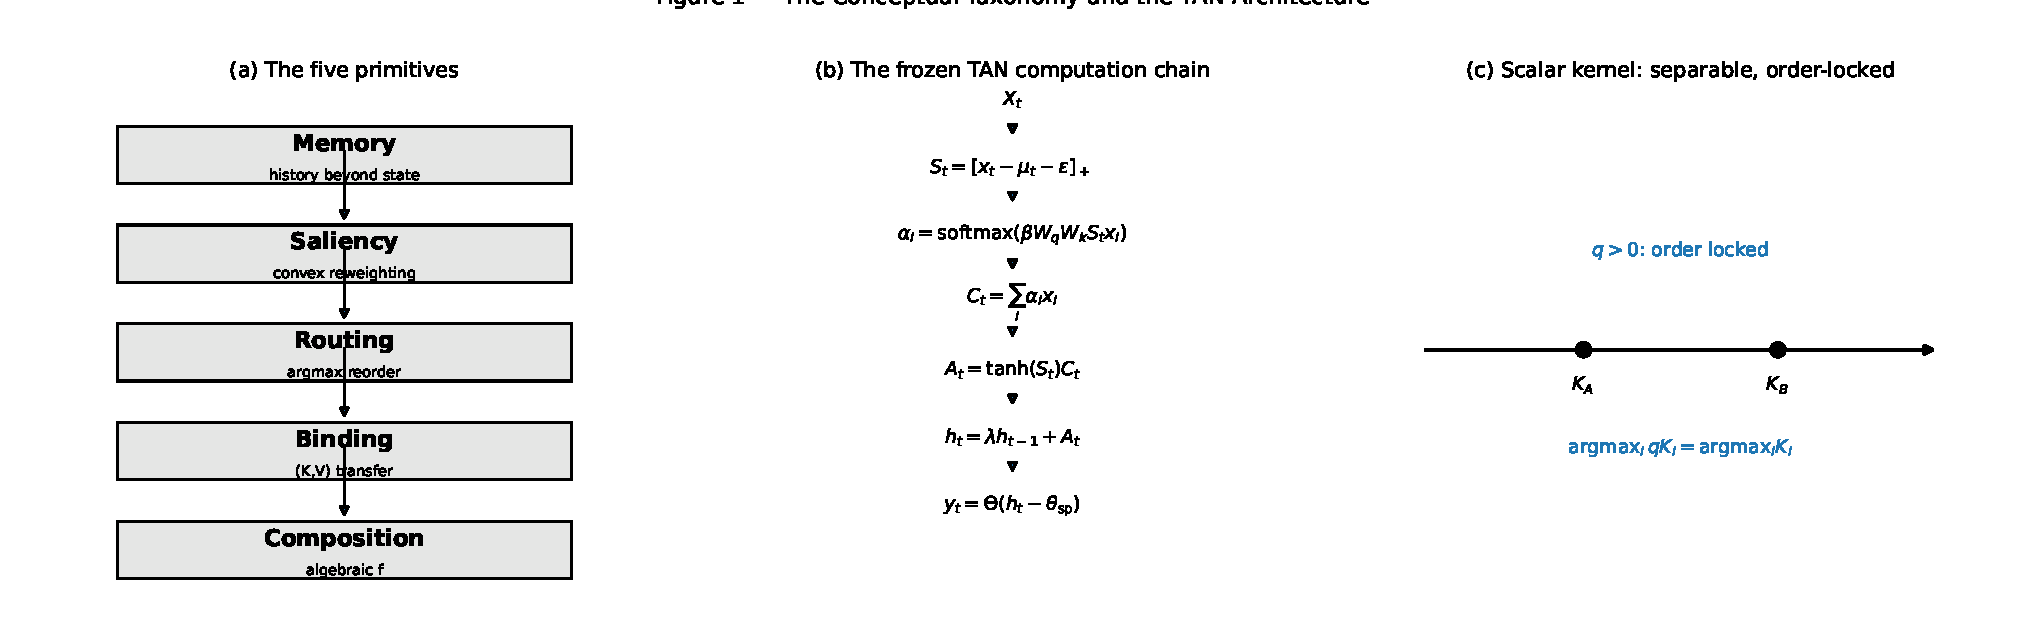
\includegraphics[width=\textwidth]{fig1_taxonomy}
\caption{The conceptual taxonomy and the frozen TAN architecture.
(a) The five primitives of §2.2 as a constructive chain. (b) The frozen
TAN-I computation chain (§2.3). (c) The degenerate geometry of the scalar
kernel: the non-negative query cone $\mathcal{Q}_+$ leaves the candidate
ordering locked to the key magnitudes (Theorem 5.1).}
\label{fig:taxonomy}
\end{figure}

\subsection{The catalog of extension operators}
\label{sec:operators}

Each rung of the ladder is one of the following operators, applied to the
baseline and left unchanged afterwards. No rung changes anything except the
named operator.

\begin{description}[style=nextline,leftmargin=2em]
\item[O1 --- Opponent competition (Sprint 4.1).] Two cells with membrane
potentials
$h_E(t)=\lambda_E h_E(t-1)+A_E(t)-w_{EI}A_I(t)$ and
$h_I(t)=\lambda_I h_I(t-1)+w_{IE}A_E(t)-w_{II}A_I(t)$, where $A_E,A_I$ are
the per-branch drives (attention-gated contexts in the attended models;
static thresholded currents $[w_E x_t-\theta_E]_+$, $[w_I x_t-\theta_I]_+$
in the static control C1) and all couplings obey Dale's sign structure
$w_{ab}\ge0$. The four-model ablation ladder C1$\to$C2$\to$C3$\to$C4 of
§4 instantiates this operator.
\item[O2 --- Vector query--key interaction (Sprint 4.2-B).] Keys are
embedded as unit vectors $\hat\varphi_d(x)=p_d(x)/\|p_d(x)\|$ with
$p_d(x)=(x,x^2,\ldots,x^d)$ and $\hat\varphi_d(0)=0$; the query is the
rotating vector $Q_t=c\,S_t\,\hat u(\theta_t)$ with angle $\theta_t=\omega S_t$ and
$\hat u(\theta)=(\cos\theta,\sin\theta,0,\ldots)$; the kernel becomes
$E_{t,i}=Q_t^{\top}K_i$. Only the representation changes: window, surprise
gate, dynamics, and readouts are frozen.
\item[O3 --- Key--value decoupling (Sprint 4.2-C).] Each slot carries a
pair $(k_i,v_i)$: keys drive the attention, values are transmitted,
$C_t=\sum_i\alpha_{t,i}v_i$. Query slots carry $v=0$ and are never
candidates.
\item[O4 --- Readout discreteness (Sprint 4.2-D).] The selection function
$\alpha_i(\gamma)=\operatorname{softmax}_i(\gamma\cdot\mathrm{logit}_i)$
with $\gamma\in[1,\infty]$; $\gamma=\infty$ is the one-hot
winner-take-all.
\item[O5 --- Parallel channels and the combiner (Sprint 4.3-A).] The
frozen window is replaced by the dual-query window $[A,0,B,Q_1,Q_2]$ with
$(Q_1,Q_2)=(4.5,5.3)$ (the direction-targeting derivation is frozen in the
pre-registration); channel $c\in\{1,2\}$ is keyed to slot $3+c$ with the
shared window mean, and a two-input node computes $y=f(\hat C_1,\hat C_2)$
with $f\in\{+,-\}$.
\end{description}

\subsection{Audit methodology and discipline}
\label{sec:audit}

Every rung is established or rejected by the following machinery, which is
itself part of the frozen protocol and is reported in §10 together with the
claim ledger.

\emph{Counterfactual suites.} A result is claimed only if it survives the
counterfactual manipulations of its rung: query swap, value swap, key swap,
channel-output swap, position randomization, amplitude randomization, the
single-query controls, and the leakage checks ($Q\cap V=\varnothing$;
queries are never candidates; equal-norm keys). Subtraction provides the
non-commutative operator whose swap responses are antisymmetric, addition
the commutative one whose swap responses are invariant---both predictions
are tested, so that correct commutative behavior can never be scored as a
false negative.

\emph{The three-error joint audit.} Composition success requires
$E_{\mathrm{bind},A}\approx0$ \emph{and} $E_{\mathrm{bind},B}\approx0$
\emph{and} $E_{\mathrm{comp}}=|y-f(V_A,V_B)|\approx0$ simultaneously. The
joint requirement exists to exclude the accidental-zero class of false
positives exemplified by the $V_A=0$ trap of §8, in which the composition
error vanishes while a binding error remains.

\emph{Negative-control chains and orthogonal axes.} Each positive claim is
paired with the demonstration that the previous rung fails the same
criterion ($M_0$ fails composition, $M_1$ binds but does not compose,
$M_2$ composes). Two orthogonal axes are formalized from these chains:
\emph{routing selectivity $\perp$ readout discreteness} (§7: the WTA ladder
changes discreteness while the flip rate stays exactly flat) and
\emph{binding fidelity $\perp$ combiner error} (§8: the combiner adds zero
error conditioned on correct binding).

\emph{Statuses and stop rules.} Every check receives an explicit
\PassFailInconclusive{}. Discrepancies with frozen predictions trigger the
stop-and-debug procedure: stop, independently recompute, record the cause in
a dated amendment that preserves the original prediction verbatim, and only
then continue. The six amendments of this programme (AM1--AM6: the E4(iii)
closed-form value, the unnormalized-control expectation, the corrected
fixed-point constants, the E-I drive-transfer value, the readout-softness
monotonicity, and the canonical routing margins) are all recorded this way;
none altered a model, query, seed, or threshold.

\emph{Determinism and statistical criteria.} All experiments are
deterministic under the fixed seeds $20260904$--$20260906$ ($N=10^4$ per
seed); analytic benchmarks are deterministic $2001^2$ quadratures computed
from the frozen model. Probability estimates are accepted when
$|\hat p-p_{\mathrm{bench}}|\le3\,\mathrm{SE}+0.002$ and mean-value
estimates when $|\hat m-m_{\mathrm{bench}}|\le3\,\mathrm{SE}_{\mathrm{mean}}
+0.01$; structural identities (swap antisymmetry, position invariance,
conditioned composition error) are asserted at machine precision
($10^{-12}$).

% ==========================================================================
% Paper 2 — Section 3: From State to Geometry. Representation Without
% Selectivity (TAN-I Phase 1 and Phase 2, frozen).
% ==========================================================================
\section{From State to Geometry: Representation Without Selectivity}
\label{sec:geometry}

This section records the two frozen TAN-I results that anchor the bottom of
the ladder: the scalar \TAN{} has genuine \emph{memory} (its state is not
Markov-sufficient), and its attention genuinely \emph{reorganizes} the
event-locked response geometry---yet neither property grants the unit any
content selectivity. The numbers are quoted verbatim from the frozen TAN-I
archive; the section proves nothing new and re-runs nothing.

\subsection{The state question: memory as non-Markovianity}
\label{sec:state}

The natural-collision experiment of TAN-I Phase~1 asks whether the pair
$(h_t,X_t)$ can be reduced to $h_t$: whether two histories that produce the
same instantaneous membrane potential are thereafter indistinguishable.
Over $N=160{,}000$ simulated histories, four model variants---B1 (leaky
integrate-and-fire), B2 (LIF with a fixed delay line), B3 (\TAN{} without
attention, $\alpha_i\equiv1/W$), B4 (the full scalar \TAN{})---and the input
control C0 were scanned for \emph{natural collisions}: pairs of histories
whose membrane states coincide while their window contexts differ. For each
pair a state-separation statistic $K$ measures how far the two futures
diverge under the identical future input.

The frozen summary is: mean $K$ is $0.5$ \emph{exactly} for B1 (maximum
deviation $1.8\times10^{-8}$, the Markov bound), $4.47\times10^{3}$
[95\% CI $3.26$--$5.92\times10^{3}$] for B2, $1.235\times10^{4}$
[$7.78\times10^{3}$--$1.83\times10^{4}$] for B3, and
$2.047\times10^{4}$ [$1.12$--$3.57\times10^{4}$] for B4 (with corresponding
medians of $0.5$, $895.5$, $1369.1$, and $2947.7$), with
$1{,}500$ pairs analysed per model; the fraction of pairs exceeding the
Markov scale $K>10^{3}$ is $0\%$ / $46.7\%$ / $56.7\%$ / $73.7\%$, and
the post-reset Markov-violation rate is $0\%$ / $0.6\%$ / $33.1\%$ /
$32.2\%$. Two controls certify the attribution: with the surprise gate
closed, the B4 median collapses to the Markov value $0.5$ (the memory lives
in the gated context, not in the leak), and a re-synchronisation test on
$n=843$ fully resynchronised pairs shows the LIF remaining synchronised
while the \TAN{} variants re-bifurcate. The state-separation statistic
correlates with the input-driven activity difference
(Pearson $r(\mathrm{JSD},\Delta A)=0.87$--$0.89$, $p<10^{-300}$).

We state the frozen consequence as a lemma.

\begin{lemma}[State insufficiency of the scalar TAN]
\label{lem:state}
The projection $\pi:(h_t,X_t)\mapsto h_t$ is not lumpable for the frozen
scalar TAN (B4): there exist histories $X_t\neq X'_t$ with
$h_t=h'_t$ whose conditional futures differ. Equivalently, the effective
state of the unit includes history content beyond the membrane potential;
the system must be treated as history-dependent throughout, and every
``phase portrait'' constructed below is conditional on a frozen history
context.
\end{lemma}

Lemma~\ref{lem:state} certifies the first rung: the substrate has memory
(primitive P1 of §2.2). It also licenses the conditional-vector-field
methodology used in §4: nothing downstream may pretend the scalar unit is
an autonomous low-dimensional system.

\subsection{The geometry question: event-locked effective dimension}
\label{sec:effdim}

TAN-I Phase~2 asked the next question in ladder order: granted memory and
saliency weighting, does attention \emph{reorganize} the unit's response
space? The frozen protocol locks the response to an event and measures an
effective response dimension $d_D$ of the event-locked fluctuation
covariance, together with its log-trace $\log\operatorname{Tr}$ as a scale
statistic (seeds 20260904--06, $T=5{,}000$, $n=374$ events). The frozen
event-velocity values are: B4 (full \TAN{}) at its content-rich frame zF
reaches $d_D=2.089$ [95\% CI $1.87$--$2.30$], versus B3 (no attention)
$d_D=1.484$ [$1.42$--$1.53$]; the plain LIF B1 and the input control C0
sit at $1.674$ and $1.055$. The amplitude-control ladder (raw /
stratified / residual) gives B4-zF $2.089$ / $2.250$ / $2.280$, and the
B4$-$B3 contrast survives all three amplitude controls
($+0.605$ / $+0.742$ / $+0.782$). In scale units the event log-trace is
$3.58$ nats for B4-zF versus $2.48$ nats for B3-zF (absolute difference
$+1.09$ nats); the frozen audit's paired delta statistic is
$\Delta\log\operatorname{Tr}(\mathrm{B4}-\mathrm{B3},\mathrm{zF})
=1.355$ nats. The effect peaks at lag $\tau\approx4$--$6$ (content-rich
windows, peak $d_D\approx2.89$), not at the first pulse, and decays with
an e-folding time $\tau_e=5.4$ [$4.6$--$6.3$] for B4 versus $8.5$
[$6.1$--$10.6$] for B3: attention sharpens and \emph{shortens} the
event-locked response.

One negative control is decisive for the ladder. In the shared frame where
B1 and B4 are compared on equal footing, B4 is \emph{not} above B1---the
attention gain is a reorganization relative to the attentionless \TAN{},
not a dimension premium over the bare LIF. We carry this asymmetry forward:
it is the first instance of the paper's rule that a geometric change must
not be read as a capability change without a boundary test.

\subsection{Interpretation discipline: effective rank is not intrinsic
dimension}
\label{sec:discipline}

The frozen archive is explicit about what Phase~2 does \emph{not} license.
$d_D$, the log-trace, and the spectra are estimator-level descriptions of
local fluctuation covariance; they are \emph{not} intrinsic manifold
dimensions, and no capacity conclusion follows from them. Attention
reshapes the event-locked response geometry---it does not, by that fact,
select content. The correct summary of the bottom two rungs is therefore:
memory (Lemma~\ref{lem:state}) and saliency weighting are realized, their
joint effect on the response space is real and measurable, and
\emph{selectivity is absent}: nothing in §3 reorders any candidate under
any query. The wall that separates this state of affairs from routing is
the subject of §4--§5.

% ==========================================================================
% Paper 2 — Section 4: Competition Without Routing. The E-I Necessity
% Counterexample (TAN-II Sprint 4.1, frozen).
% ==========================================================================
\section{Competition Without Routing: The E-I Necessity Counterexample}
\label{sec:competition}

The first candidate degree of freedom above scalar saliency is opponent
competition: an excitatory--inhibitory microcircuit with Dale's sign
discipline. This section reports the frozen Sprint 4.1
ablation ladder C1$\to$C2$\to$C3$\to$C4 and its two outcomes: opponent
topology suffices, by an analytic open-set theorem, for nonmonotonic
selective tuning---\emph{without any attention at all}; and it does
nothing whatsoever to the routing boundary.

\subsection{The opponent mechanism and its open-set theorem}
\label{sec:opponent}

Consider the static opponent readout on a scalar input $x\in[0,x_{\max}]$,
\begin{equation}
R(x)=[w_E x-\theta_E]_+ - g\,[w_I x-\theta_I]_+,
\qquad w_E,w_I,\theta_E,\theta_I,g\ge0,
\label{eq:opponent}
\end{equation}
the instantaneous (pre-leak) form of the two-cell circuit used in §4.3.
Its three regimes have slopes $0$ (silence, $x<\theta_E/w_E$),
$w_E>0$ (excitation only), and $w_E-g\,w_I$ (both active). The frozen
inequalities single out the regime in which the second slope is negative.

\begin{theorem}[E-I nonmonotonicity]
\label{thm:EI}
Let
$U=\{(w_E,w_I,\theta_E,\theta_I,g):\ \theta_E/w_E<\theta_I/w_I<x_{\max},
\ g\,w_I>w_E\}$. For every parameter point in the open set $U$, the
readout \eqref{eq:opponent} has a strict local maximum at
$x^*=\theta_I/w_I$: the left slope is $w_E>0$ and the right slope is
$w_E-g\,w_I<0$. The maximum is strict and persists under the leaky
embedding $h^*(x)=R(x)/(1-\lambda)$ with $0\le\lambda<1$.
\end{theorem}

\begin{proof}
On $(\theta_E/w_E,\theta_I/w_I)$ only the first branch is active, so
$R(x)=w_E x-\theta_E$ with slope $w_E>0$; on
$(\theta_I/w_I,x_{\max})$ both branches are active and
$R(x)=(w_E-g w_I)x-\theta_E+g\theta_I$ with slope $w_E-g w_I<0$ by the
second inequality of $U$. Continuity at $x^*$ follows from
$[w_I x^*-\theta_I]_+=0$, so $R$ is a continuous, piecewise-linear map that
rises into $x^*$ and falls away from it: a strict local maximum. Division
by the positive constant $1-\lambda$ preserves the sign of every slope.
\end{proof}

With the frozen constants $(w_E,w_I,\theta_E,\theta_I,g)=
(0.5,1.0,0.4,1.0,0.8)$ the conditions read
$0.8<1.0<3.0$ and $0.8\cdot1.0>0.5$, the peak sits at $x^*=1.00$ with
height $h_E^*=0.200$, and the leaky slopes are $+1.0$ and $-0.6$
(rising slope $w_E/(1-\lambda)$, falling slope
$(w_E-g w_I)/(1-\lambda)$, $\lambda=0.5$).

\begin{remark}
The theorem is the paper's first necessity counterexample: it certifies
that a local tuning peak exists in a configuration with \emph{zero
attention}, zero surprise gating, and zero temporal organization. Any
later observation of nonmonotone selectivity inside an attended
configuration therefore \emph{cannot} be attributed to attention unless
the attended rungs change the peak itself.
\end{remark}

\subsection{The C1--C4 ablation ladder: what attention actually adds}
\label{sec:ladder41}

The frozen four-rung ladder instantiates the operator O1 of §2.4 inside
the conditional fixed-point readout of Lemma~\ref{lem:state}: C1, the
static E-I LIF (drives $[w_E x_t-\theta_E]_+$, $[w_I x_t-\theta_I]_+$, no
surprise, no window attention); C2, the \TAN{} with surprise gating and
forced uniform attention ($\alpha_i\equiv1/W$); C3, asymmetric attention
(E-branch attends, I-branch integrates uniformly); C4, the full classical
E-I \TAN{} (both branches with independent surprise and attention). The
pre-registered monotonicity criterion P1 (finite-difference sign flip plus
curvature, tolerances $10^{-3}$/$2\times10^{-3}$/$5\times10^{-3}$, spike
adjacency excluded) was applied to the conditional fixed point
$h_E^*(x^*)$ over the probe range $x^*\in[0.2,3.0]$ (57 points,
$\delta=0.05$), and every prediction was frozen before the run.

The frozen verdicts: C1 \textbf{PASS} (peak at $x^*=1.00$, height
$0.200$, prominence $0.100$, curvature $-0.11$, post-peak suppression slope
$-0.600$ with $R^2=1.0$, maximal suppression $1.200$); C2 \textbf{FAIL}
(climb-then-plateau: maximum $0.5595$ at $x^*=1.80$ decaying only to
$0.5344$ at $3.0$, a $0.025$ plateau modulation below the curvature
tolerance); C3 \textbf{FAIL} (monotone climb to $3.8897$ at $3.0$, spike
onset $2.60$, $15.8\%$ of the scan in the spiking regime); C4
\textbf{FAIL} (monotone climb to $1.3592$ at $3.0$, subthreshold
throughout). The episodic-protocol cross-checks reproduce every verdict,
and the six-layout robustness sweep reproduces them layout by layout
(C1 PASS, C2--C4 FAIL everywhere). The prediction table was hit $4/4$.

The causal reading is forced by the ladder and is one of the paper's
central re-definitions. \emph{Nonmonotone selectivity comes from the
opponent threshold structure (C1), not from attention:} the attended rungs
C2--C4 do not produce a single strict peak under the frozen criteria.
What attention demonstrably does at each rung is gain and operating-range
modulation: the surprise gate rectifies and saturates (C1's negative
inhibitory tail disappears, replaced by the C2 plateau); E-only attention
amplifies gain until the unit enters the spiking regime (C3); and
symmetric E/I attention re-reads the probe through the inhibitory branch
and pulls the net response back into the subthreshold band (C4). Attention
is thus a \emph{dynamic gain and operating-point regulator} in this
substrate---not a source of selectivity, and not a router.

\begin{figure}[t]
\centering
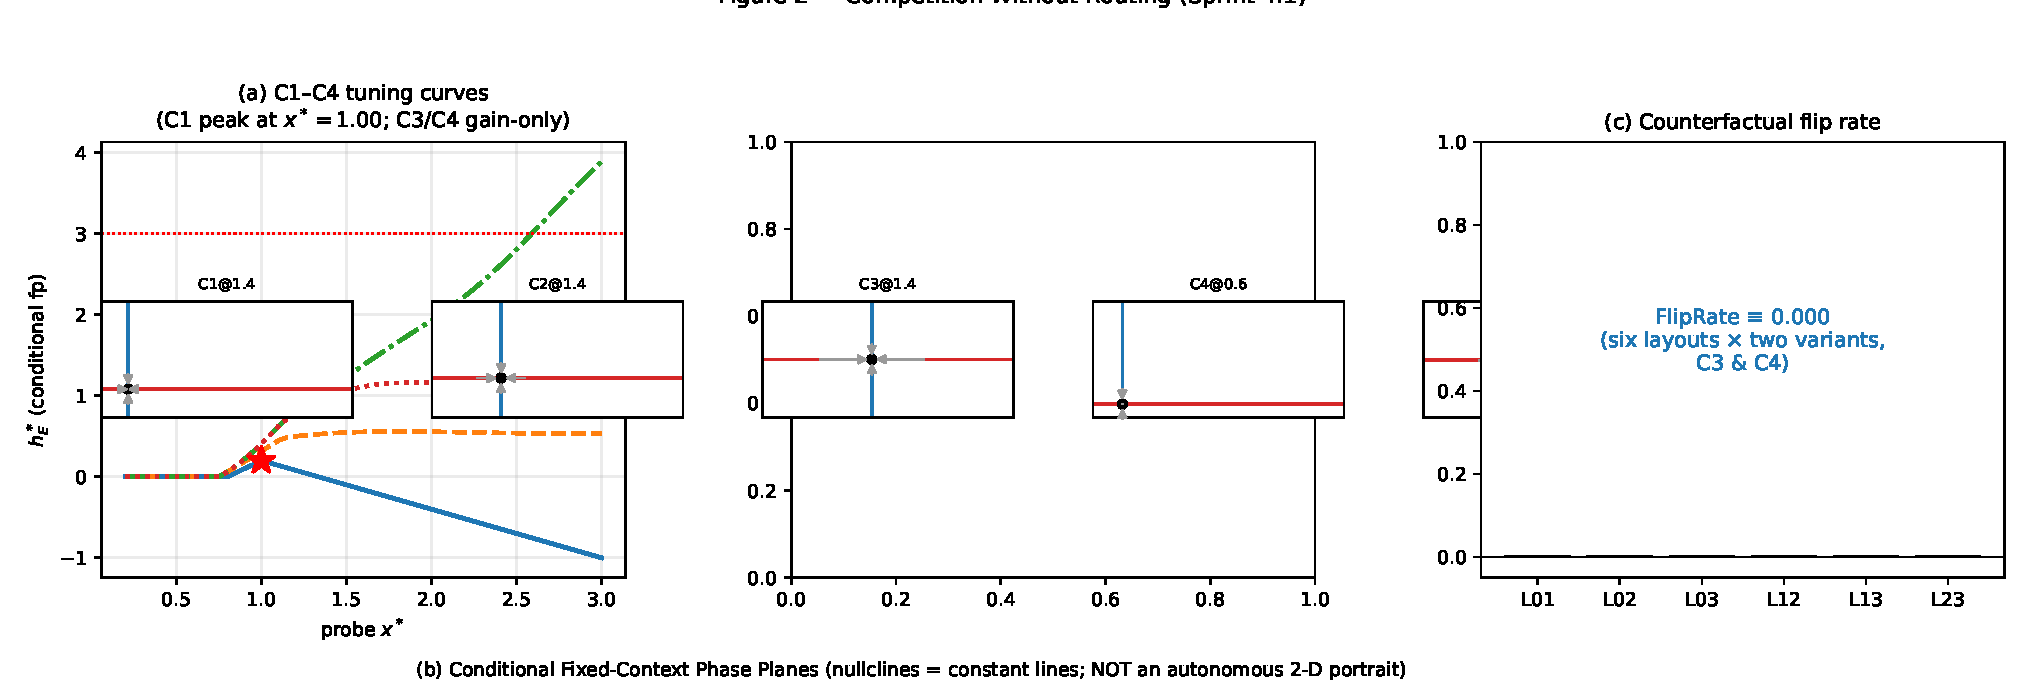
\includegraphics[width=\textwidth]{fig2_competition}
\caption{Competition without routing (Sprint 4.1). (a) The C1--C4
conditional-fixed-point tuning curves: only the static opponent model C1
exhibits a strict local maximum ($x^*=1.00$, $h_E=0.200$); the attended
rungs C2--C4 only reshape gain. (b) Conditional fixed-context phase
planes: the conditional nullclines are the constant lines
$h_E=h_E^*$, $h_I=h_I^*$; they are \emph{not} an autonomous two-dimensional
portrait. (c) The counterfactual flip rate is exactly $0.000$ across all
six layouts and both variants.}
\label{fig:competition}
\end{figure}

\subsection{Conditional phase planes, honestly labeled}
\label{sec:phaseplanes}

For completeness the frozen sprint also froze the conditional vector
fields: for a frozen history context $X^*$ and a frozen probe $x^*$ the
drives $A_E(X^*,x^*)$, $A_I(X^*,x^*)$ are constants, so the subthreshold
flow is the affine contraction
$h_a(t)=\lambda_a h_a(t-1)+B_a(X^*,x^*)$ with conditional fixed points
$h_E^*=B_E/(1-\lambda_E)$, $h_I^*=B_I/(1-\lambda_I)$ and conditional
nullclines that are the \emph{constant lines} $h_E=h_E^*$,
$h_I=h_I^*$. Every figure in the frozen archive labels these
``Conditional Fixed-Context Phase Plane'' and states explicitly that they
are \emph{not} an autonomous two-dimensional phase portrait; different
probe values translate the affine field rather than deform an intrinsic
topology, and any probe whose fixed point crosses the spike threshold is
flagged as a spiking regime. No claim of two-dimensional autonomous
dynamics is made anywhere in this paper.

\subsection{The routing boundary survives competition}
\label{sec:flip41}

The counterfactual criterion P2 (fixed history, queries $Q_A=3.0$,
$Q_B=4.0$, winner = attention argmax over history candidates, two
variants) was run across all six event layouts. The frozen outcome is
$\mathrm{FlipRate}\equiv0.000$ in every layout, every variant, and every
attended model (C3, C4; C1/C2 have no candidate structure and were
pre-registered as not applicable), while the response magnitude is
query-sensitive ($\Delta R=+1.827$ for C3, $+0.281$ for C4). The spike
threshold sweep ($\theta_{\mathrm{sp}}\in\{0.5,1.0,3.0,6.0\}$) documents
the spiking onsets (e.g.\ C3 at $2.60$ for the default $3.0$; C2/C3/C4 at
$1.25/1.05/1.05$ for the TAN-I threshold $0.5$) and shows that the
monotonicity verdicts live entirely in the subthreshold region and are
threshold-robust. The structural reason for the flat zero is recorded for
later use: the winner is decided by the kernel's argmax \emph{before} any
E-I dynamics, and opponent competition acts on the scalar aggregate
$C=\sum_i\alpha_i v_i$, which cannot reorder candidates. The boundary to
be crossed is therefore not dynamical but representational, which is
precisely what the next rung changes.

\[
\boxed{\ \text{E-I Competition}\ \not\Rightarrow\ \text{Content Routing}\ }
\]

% ==========================================================================
% Paper 2 — Section 5: The Geometric Boundary of Routing. Hyperplane
% Bisection in d=2 (TAN-II Sprints 4.2-A / 4.2-B, frozen).
% ==========================================================================
\section{The Geometric Boundary of Routing: Hyperplane Bisection in
\texorpdfstring{$d=2$}{d=2}}
\label{sec:routing}

Section 4 closed the dynamical avenue: opponent competition reshapes
tuning and gain but cannot reorder candidates, because ordering is decided
by the kernel before any downstream dynamics. The boundary is therefore
representational, and this section crosses it with the minimal
representational change---operator O2 of §2.4, the vector query--key
interaction. The section proceeds in four parts: the exact theorem that
explains why the scalar lineage was locked (the order-conservation
theorem); the pure geometry of hyperplane bisection and its exact flip
law $\mathrm{FlipRate}_{\mathrm{CF}}(\theta)=\theta/\pi$; the
ordering-capacity ladder that generalizes the flip law beyond two
candidates; and the realization of all of this inside the running neuron
(Sprint 4.2-B), including the shortcut audits that certify the flips are
not artifacts.

\subsection{The order-conservation theorem}
\label{sec:orderconservation}

\begin{theorem}[Order conservation of the separable scalar kernel]
\label{thm:order}
Let $d=1$, $K_A\neq K_B$, and let the query domain $D\subseteq\mathbb{R}$
intersect at most one sign class of $\mathbb{R}\setminus\{0\}$. Then the
winner of the dot-product kernel $E_i(Q)=QK_i$ is constant on $D$:
$w(Q)=\operatorname{argmax}_i K_i$ for $D\subseteq(0,\infty)$ and
$w(Q)=\operatorname{argmin}_i K_i$ for $D\subseteq(-\infty,0)$. In
particular, for the frozen TAN kernel $E_{t,i}=\beta W_qW_kS_tx_i$ the
query $q_t=\beta W_qW_kS_t$ lies in the closed cone $\mathcal{Q}_+=
[0,\infty)$, so $\operatorname{argmax}_i E_{t,i}=\operatorname{argmax}_i
x_i$ for every active query, and the counterfactual flip rate is exactly
zero.
\end{theorem}

\begin{proof}
$QK_A>QK_B\iff (Q>0 \wedge K_A>K_B)\vee(Q<0\wedge K_A<K_B)$, so the winner
is constant on each sign class and changes only when the query crosses
zero. The \TAN{} query never does: $S_t=[x_t-\mu_t-\varepsilon]_+\ge0$ and
$\beta,W_q,W_k>0$.
\end{proof}

Theorem~\ref{thm:order} is the paper's sharpest statement of the wall that
Sprint 4.2-A had to audit, and it is deliberately \emph{domain-conditional}:
a signed scalar query ($D=\{+1,-1\}$) \emph{can} flip the winner, but only
by the degenerate global reversal $w(-1)=\operatorname{argmin}_iK_i$, a
one-bit, order-locked capacity (flip rates confined to $\{0,1\}$). The
correct universal claim is therefore never ``one-dimensional attention
cannot route'' but: \emph{within the positive-query scalar family inherited
from TAN-I, candidate ordering is query-invariant}. This scoping is frozen
as Amendment AM1 of the programme and is used verbatim here.

\subsection{Hyperplane bisection and the flip law}
\label{sec:bisection}

Fix two candidates $K_A,K_B\in\mathbb{R}^d$ ($d\ge2$) with
$\Delta K=K_A-K_B\neq0$, and sample the query isotropically,
$Q\sim\mathrm{Unif}(S^{d-1})$. The decision boundary
$\mathcal{H}_0=\{Q:Q^{\top}\Delta K=0\}$ is a hyperplane through the
origin, i.e.\ a great $(d-2)$-sphere on $S^{d-1}$, so it bisects the query
sphere into two open hemispheres of equal measure---\emph{regardless of the
candidate norms}, because the boundary is homogeneous.

\begin{proposition}[Equal bisection]
\label{prop:bisection}
For any $K_A\neq K_B$ and isotropic $Q$ on $S^{d-1}$,
$\Pr_Q[w(Q)=A]=\Pr_Q[w(Q)=B]=\tfrac12$.
\end{proposition}

\begin{proof}
$\Pr[Q^{\top}\Delta K>0]=\Pr[Q\cdot\hat u>0]$ with
$\hat u=\Delta K/\|\Delta K\|$; the projection of a uniform unit vector
onto a fixed axis is symmetric about zero.
\end{proof}

\begin{corollary}[Dimension-independent winner variation]
\label{cor:fd}
For i.i.d.\ queries $Q_1,Q_2$,
$F_d=\Pr[w(Q_1)\neq w(Q_2)]=2\cdot\tfrac12\cdot\tfrac12=\tfrac12$ for
every $d\ge2$; the same holds for the signed scalar ($d=1$, uniform on
$\{\pm1\}$), while the positive scalar lineage gives $F_d=0$. The Monte
Carlo estimates freeze at $0.4996/0.4997/0.5033/0.4998$ for
$d=2,3,4,8$: \emph{higher dimension does not mean stronger routing}, and
$F_d$ is retained in this paper only as a negative control, never as a
transition statistic.
\end{corollary}

The counterfactual quantity that \emph{does} carry the geometry is the flip
rate of a fixed query pair over randomized histories. Let the history be
isotropic, $\Delta K\sim\mathrm{Unif}(S^{d-1})$, and fix two queries
$Q_A,Q_B\in S^{d-1}$ with angular separation
$\theta=\arccos(Q_A^{\top}Q_B)\in[0,\pi]$.

\begin{proposition}[The flip law]
\label{prop:fliplaw}
$\mathrm{FlipRate}_{\mathrm{CF}}(\theta)
=\Pr_{\Delta K}\bigl[w(Q_A)\neq w(Q_B)\bigr]=\theta/\pi$.
\end{proposition}

\begin{proof}
Rotate so that $Q_A=e_1$, $Q_B=\cos\theta\,e_1+\sin\theta\,e_2$. A flip
occurs iff $(\Delta K_1)\bigl(\cos\theta\,\Delta K_1+\sin\theta\,\Delta
K_2\bigr)<0$. Writing $\Delta K_1=r\cos\phi$, $\Delta K_2=r\sin\phi$, the
marginal law of $(\Delta K_1,\Delta K_2)$ is rotationally symmetric in the
$(1,2)$-plane, so $\phi$ is uniform on $[0,2\pi)$, and the event is
$\cos\phi\cos(\phi-\theta)<0$, the union of two arcs of angular width
$\theta$: total measure $2\theta$ out of $2\pi$.
\end{proof}

The frozen verification is exact at both levels. Analytically, a
root-decomposition of the indicator reproduces $\theta/\pi$ on the full
11-point angle grid (endpoints $0\to0$, $\pi\to1$) at machine precision,
independently of the closed form (connecting to the classical random
hyperplane flip law of \citet{charikar2002}); and the Monte Carlo
audit---$d\in\{2,3,4,8\}\times11$ angles $\times3$ seeds, $132/132$
conditions, maximum deviation across 3-seed averages $0.004667$ (maximum
single-seed absolute deviation $0.009267$; grid parameter recorded as
$\theta/\pi$)---agrees with the curve point by point. The
degenerate endpoints of the scalar lineage sit exactly where the theorem
predicts: the signed scalar realizes only $\{0,1\}$ (queries equal or
opposite), the positive scalar only $\{0\}$. The transition recorded in
this section is therefore not ``$d=1\to d=2$ increases flips'' but the
topological change $S^{0}\to S^{1}$: the query-direction manifold becomes
connected, and the flip rate becomes a continuous function
$\theta/\pi\in[0,1]$ of a continuous query angle.

\subsection{The ordering-capacity ladder}
\label{sec:capacity}

The pairwise flip law extends to a capacity statement over $M$ candidates.
For $M$ keys in general position, the achievable orderings of
$(Q^{\top}K_1,\ldots,Q^{\top}K_M)$ as $Q$ ranges over the query domain are
the cells of the central arrangement of the $C(M,2)$ difference
hyperplanes. Frozen exact computations (arrangement enumeration, linear
programming existence, and a $200{,}000$-angle dense sampling cross-check)
establish the ladder:

\begin{center}
\begin{tabular}{@{}lcccc@{}}
\toprule
$M$ & positive scalar & signed scalar & $d=2$ & $d=3,8$ \\
\midrule
2 & 1 & 2 & 2 & 2 \\
3 & 1 & 2 & 6 & 6 \\
4 & 1 & 2 & 12 & 24 \\
\bottomrule
\end{tabular}
\end{center}

\noindent i.e.\ $1$ / $2$ / $M(M-1)$ / $M!$ (the last for $M\le d+1$ in
general position). Two facts anchor the paper's reading. First, the signed
scalar is stuck at two orderings for \emph{every} $M$: its ``routing'' is
the global reversal of a fixed magnitude order, never a content address.
Second, $d=2$ already realizes \emph{all} $3!=6$ orderings of three
candidates, so $d=2$ is the minimal dimension for a connected,
rotationally symmetric continuous query-direction manifold---the statement
this paper is willing to make, with the qualifier that it concerns the
tested positive-scalar lineage and the tested query--key family. Higher
ambient dimension adds nothing to this pairwise or three-candidate
capacity.

\subsection{Realization in the running neuron (Sprint 4.2-B)}
\label{sec:realization}

The geometry is only half of the rung; the frozen programme demands that
the running model actually flip, under the iron gate that \emph{only the
representation changes} (window, surprise gate, membrane, readout all
frozen). Sprint 4.2-B does exactly this with operator O2
($\hat\varphi_2$ keys, rotating query $c\,S_t\hat u(\omega S_t)$,
$\omega=0.4$), and its deterministic canonical audit closed every
pre-registered prediction:

\begin{itemize}
\item \emph{Counterfactual winner flip.} Fixed history
$[1,0,2,0]$, only the query changes $3\to4$: the attention winner flips
$A\to B$ with energy margins $+0.2587427\to-0.1559101$; the crossing
$Q^*=3.7071$ matches the closed form and the winner-vs-query scan
(A for $Q\le3.70$, B for $Q\ge3.75$).
\item \emph{No amplitude-code leakage.} The probe slot's energy
($3.1078$ at $Q=3$; $4.9890$ at $Q=4$) stays \emph{below} the winning
event at both queries, in direct contrast to the scalar lineage, whose
probe dominates the window ($10.8$/$20.8$).
\item \emph{The JSD conjunction.} In a 2-candidate geometric toy example,
the scalar trap exhibits JSD$=0.0751$ with zero flip (query changes
sharpness, not order), while the vector model exhibits JSD$=0.0647$ with
a winner flip. In the full 5-slot window ($[1,0,2,0,Q]$), the canonical
distribution shifts yield full-window JSDs of $0.009462$ (M0) and $0.008727$ (M2).
\item \emph{Normalization is a mechanistic enabler.} With raw magnitude
keys the kernel reads
$(x_A-x_B)[\cos\theta+(x_A+x_B)\sin\theta]$, whose sign is fixed in the
query range: the unnormalized control has flip rate exactly $0$ (frozen
Amendment AM2), while the normalized model reaches $0.4425$ on the
randomized ensemble against the $0.4445$ quadrature benchmark
(3 seeds $\times10^4$, all within criterion).
\item \emph{Structure, not luck.} The sweep over
$\omega\in\{0.2,\allowbreak0.4,\allowbreak\pi/2,\allowbreak\pi\}$ yields
winners $(A,A)$, $(A,B)$, $(B,B)$, $(A,B)$: the flip exists exactly when
the query direction sweeps across the decision boundary, with the
closed-form crossings in place.
\item \emph{Dimension controls.} In this mechanism family, increasing the
ambient embedding dimension beyond the minimal 2-D query subspace did not
increase routing capacity and, under the tested finite
candidate/query configuration, \emph{reduced} the observed flip rate
(ensemble benchmarks $0.0549$/$0.0284$/$0.0172$ for $d=3,4,8$; canonical
flips absent). The cause is a representation--candidate geometry
mismatch---the key-difference vector leaves the 2-D query subspace and the
attention mass is absorbed by the silent slots---not a ``curse of
dimensionality''.
\end{itemize}

\begin{figure}[t]
\centering
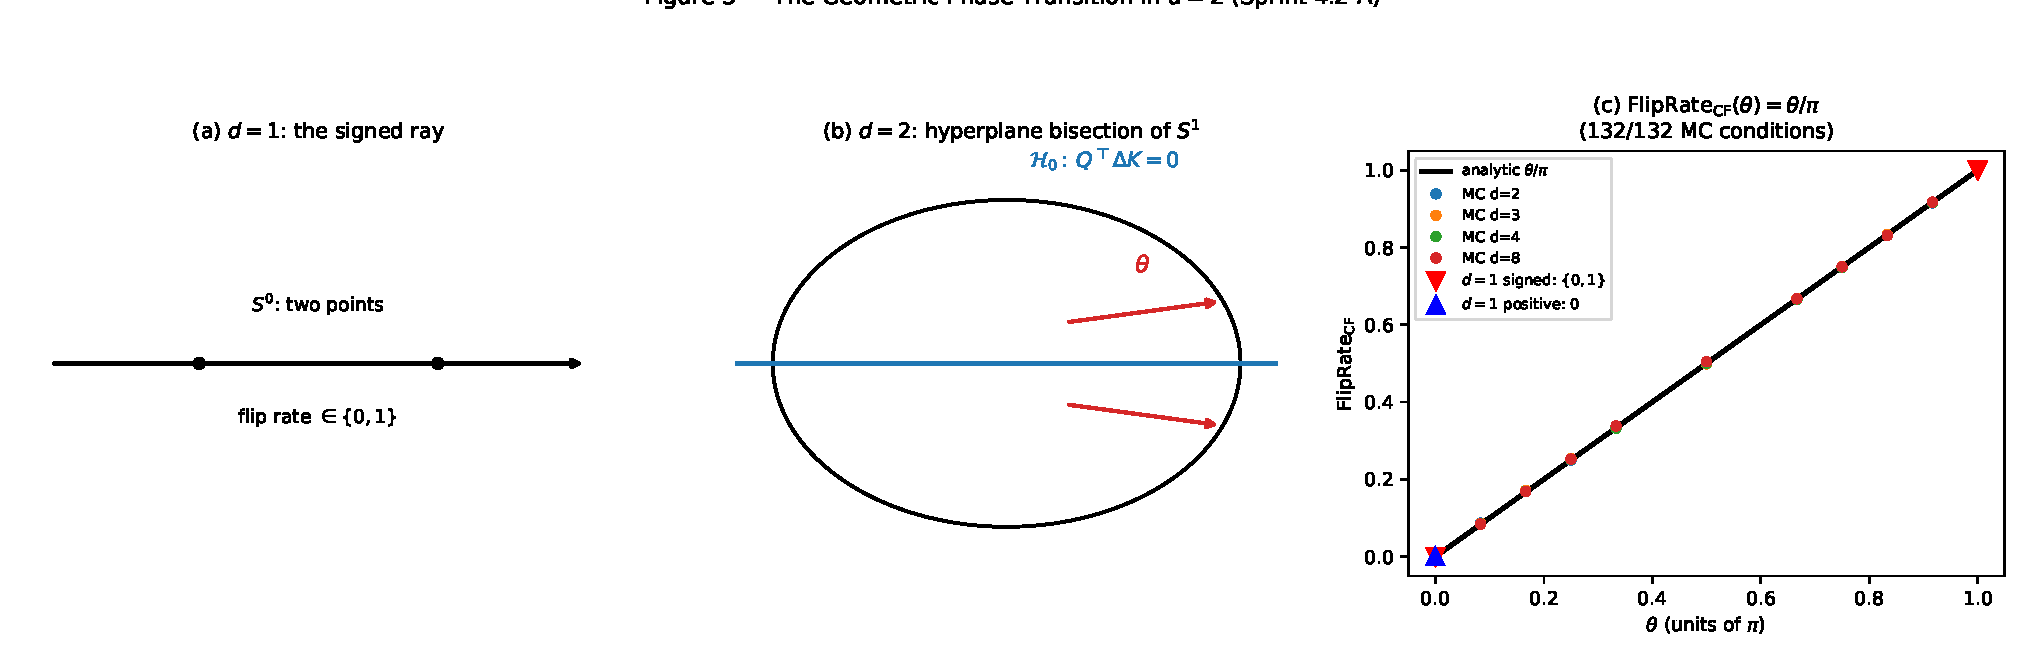
\includegraphics[width=0.66\textwidth]{fig3_phase}\hfill
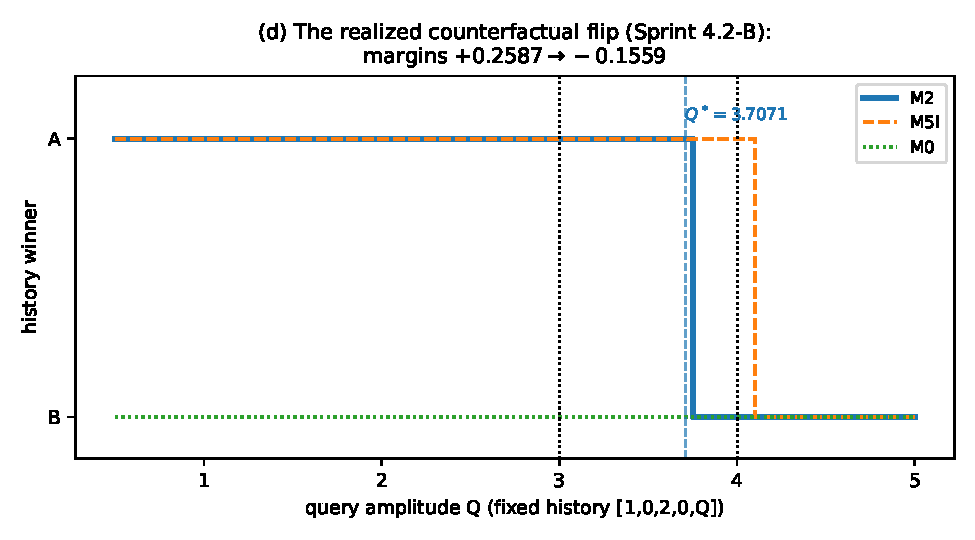
\includegraphics[width=0.32\textwidth]{fig3d_realization}
\caption{The geometric boundary of routing. (a)--(c) The pure geometry
(Sprint 4.2-A): the signed scalar ray realizes only the degenerate flip
rates $\{0,1\}$; in $d=2$ the decision hyperplane bisects the query sphere;
and the Monte Carlo flip rates sit on the analytic curve
$\mathrm{FlipRate}_{\mathrm{CF}}(\theta)=\theta/\pi$ (132/132 conditions,
$d\in\{2,3,4,8\}$). (d) The realization in the running neuron
(Sprint 4.2-B): on the fixed history $[1,0,2,0]$, changing only the query
flips the attention winner at the closed-form crossing $Q^*=3.7071$, with
margins $+0.2587\to-0.1559$.}
\label{fig:phase}
\end{figure}

\subsection{Sufficiency of 1D Metric Compatibility and the Multi-Candidate Address Identifiability Boundary}
\label{sec:metric_sufficiency}

The analysis in \S\ref{sec:orderconservation}--\ref{sec:bisection} demonstrated that within the scalar dot-product family inherited from TAN-I, candidate ordering is invariant under positive queries, and that two-dimensional rotation ($S^1$) unlocks counterfactual winner flips. This raises a fundamental theoretical and architectural question: \emph{is multidimensional representation strictly necessary for single-neuron content addressing, or was the scalar failure an artifact of separable dot-product multiplication ($E(q, k) = q \cdot k$)?}

To resolve this question definitively, we established two formal propositions and executed a comprehensive multi-candidate address identifiability audit (60,000 synthetic histories, 420,000 model evaluations across 7 model architectures and 6 conditions).

\begin{proposition}[1D Metric Sufficiency under Hard Selection]
\label{prop:metric_suff}
Let $\{k_1, k_2, \dots, k_N\} \subset \mathbb{R}$ be a set of $N \ge 2$ distinct scalar keys. Define the scalar distance compatibility kernel by $E(q, k) = -(q - k)^2$. Then for any target key $k_t$, setting the query to $q = k_t$ uniquely selects $k_t$ under hard argmax routing:
\begin{equation}
\operatorname{argmax}_{i \in \{1,\dots,N\}} E(k_t, k_i) = t.
\end{equation}
Furthermore, the selection margin is strictly positive: $\Delta E = \min_{i \ne t} (k_i - k_t)^2 > 0$.
\end{proposition}

\begin{proposition}[Impossibility of Scalar Intermediate Addressing]
\label{prop:scalar_impossible}
Let $N \ge 3$ and let $k_{(1)} < k_{(2)} < \dots < k_{(N)}$ be ordered distinct scalar keys. For any generalized scalar multiplication kernel of the form $E(q, k) = \alpha(q) \cdot k$ where $\alpha: \mathbb{R} \to \mathbb{R}$ is an arbitrary scalar function:
\begin{enumerate}[label=(\roman*)]
\item If $\alpha(q) > 0$, $\operatorname{argmax}_i E(q, k_i) = k_{(N)}$;
\item If $\alpha(q) < 0$, $\operatorname{argmax}_i E(q, k_i) = k_{(1)}$;
\item If $\alpha(q) = 0$, $E(q, k_i) \equiv 0$ for all $i$ (tie across all candidates).
\end{enumerate}
In all cases, any intermediate key $k_{(j)}$ with $1 < j < N$ cannot be selected as the unique maximum for any query $q \in \mathbb{R}$.
\end{proposition}

\begin{proof}
Direct from linearity: for any non-zero $\alpha(q)$, multiplication by $\alpha(q)$ either strictly preserves ($\alpha > 0$) or strictly reverses ($\alpha < 0$) the order of the keys. An intermediate element in a strictly ordered sequence can never become the maximum under order-preserving or order-reversing bijections.
\end{proof}

\begin{figure}[t]
\centering
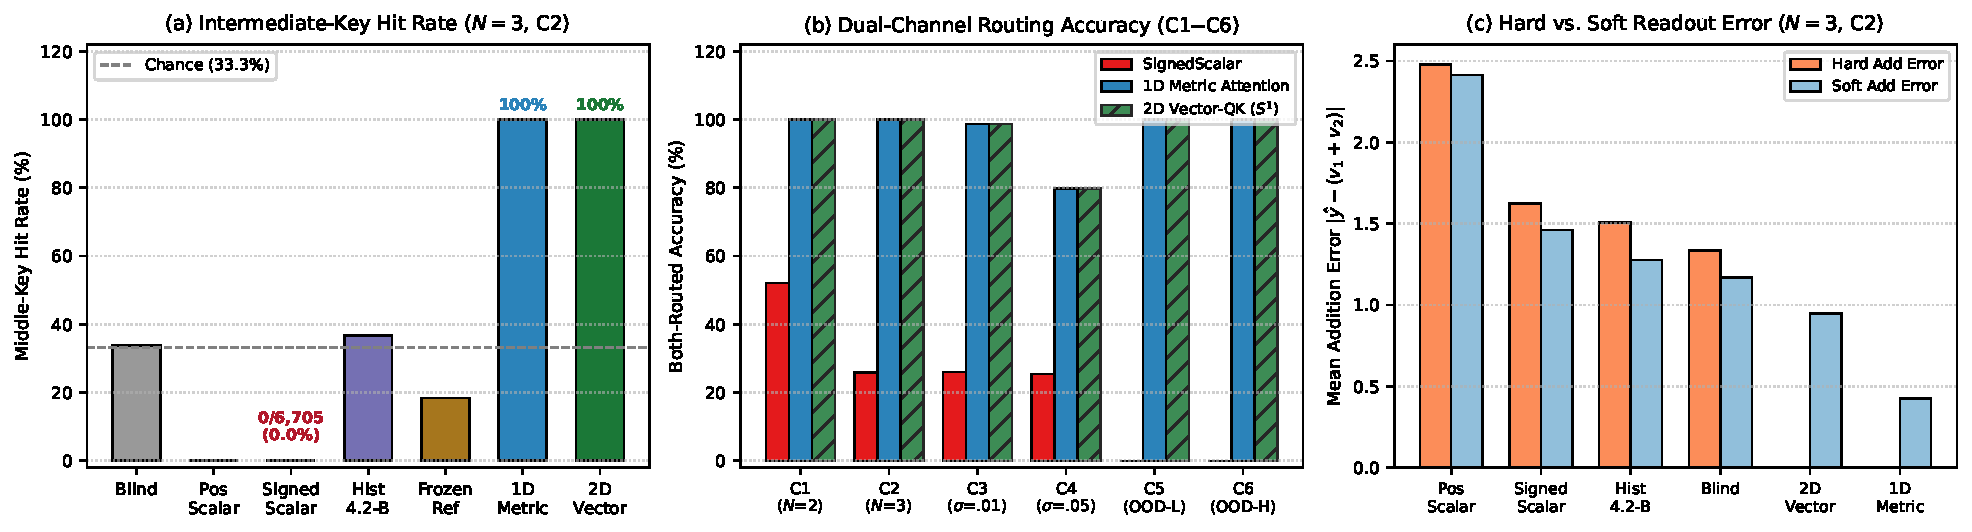
\includegraphics[width=\textwidth]{fig7_p1a_identifiability}
\caption{Address identifiability and the multi-candidate routing boundary (420,000 model evaluations). (a) On $N=3$ candidates (Condition C2), intermediate keys cannot be addressed by scalar multiplier kernels: SignedScalar achieves exactly $0/6{,}705$ hits ($0.0\%$), whereas 1D Metric Attention achieves $100.00\%$ hit rate, identical to 2D Vector-QK on $S^1$. (b) Dual-channel both-routed accuracy across clean ($N=2, 3$), noise-perturbed ($\sigma \in \{0.01, 0.05\}$), and out-of-distribution amplitude ranges (C5, C6). (c) Soft addition readout error on C2: hard routing accuracy is $100\%$ for both 1D Metric and 2D Vector-QK, but soft readout reveals residual leakage governed by kernel curvature ($0.4247$ vs.\ $0.9463$).}
\label{fig:p1a_identifiability}
\end{figure}

The empirical consequences of Propositions~\ref{prop:metric_suff} and \ref{prop:scalar_impossible} were verified across 6 experimental conditions (Figure~\ref{fig:p1a_identifiability}):
\begin{itemize}
\item \emph{Empirical refutation of 2D necessity:} On Condition C1 ($N=2$) and Condition C2 ($N=3$), the 1D Metric Attention model achieves $100.00\%$ both-routed accuracy with zero hard addition error, exactly matching the 2D Vector-QK model on $S^1$ across all 60,000 trials. This proves that 2D orthogonal rotation is \emph{not} mathematically necessary for content addressing: a 1D scalar distance metric is sufficient.
\item \emph{Empirical confirmation of the intermediate-key barrier:} In Condition C2 ($N=3$, 10,000 trials $\times$ 2 query channels), exactly $6{,}705$ channel queries targeted the intermediate key ($k_{(1)} < k_{\text{target}} < k_{(3)}$). In exact agreement with Proposition~\ref{prop:scalar_impossible}, the SignedScalar kernel achieved \textbf{exactly $0$ hits out of $6{,}705$ queries ($0.00\%$ hit rate)}, whereas 1D Metric Attention and 2D Vector-QK achieved $6{,}705/6{,}705$ ($100.00\%$).
\item \emph{Demarcation of Historical 4.2-B:} The static control model \textsc{Hist4.2-B} achieved only $13.68\%$ both-routed accuracy on C2 (middle-key channel hit rate $36.78\%$, near the $33.33\%$ blind chance level). This demonstrates that the winner flips observed in historical Sprint 4.2-B were fixed counterfactual switches between two pre-tuned surprise amplitudes, rather than true content-addressable memory retrieval.
\item \emph{Soft readout error bounds:} Under soft softmax readout, the addition error on C2 differs between 1D Metric ($0.4247$) and 2D Vector-QK ($0.9463$). For a distance metric kernel, the soft error is strictly bounded by the minimum key separation $\delta$ and temperature $\gamma$:
\begin{equation}
|\hat{v}_{\mathrm{soft}} - v_t| \le M \frac{(N-1)e^{-\gamma\delta^2}}{1 + (N-1)e^{-\gamma\delta^2}}, \qquad M = \max_{i\ne t}|v_i - v_t|.
\end{equation}
\end{itemize}

\subsection{What this section does and does not establish}
\label{sec:scope5}

The scoped claim is: \emph{within the tested positive-scalar lineage, $d=2$
is the minimal dimension for continuous query-direction freedom under dot-product kernels, and the
running neuron realizes the resulting query-conditioned reordering
(Level-2 realized routing)}. However, moving from dot-product ranking to 1D distance metric compatibility ($E = -(q-k)^2$) restores full multi-candidate content addressability without requiring higher-dimensional rotation. It is \emph{not} claimed that $d=2$ routes in
every representation family (the $d=3,4,8$ controls show the opposite for
the tested maps), nor that any flip constitutes semantic binding---that
requires the key--value decoupling of the next section---nor that anything
resembling a thermodynamic phase transition has been located: the
transition language used here is the minimal-integer-dimensional geometric
transition, not an order-parameter limit.

% ==========================================================================
% Paper 2 — Section 6: From Routing to Binding. Representation Decoupling
% (TAN-II Sprint 4.2-C, frozen).
% ==========================================================================
\section{From Routing to Binding: Representation Decoupling}
\label{sec:binding}

Routing changes \emph{which} candidate is selected; binding additionally
requires that the selected candidate's \emph{content} be transmitted, and
that the transmission follow the (key, value) association rather than key
identity, position, or amplitude. The minimal degree of freedom that
separates the two is operator O3 of §2.4: each slot now carries a pair
$(k_i,v_i)$, keys drive the attention, values are transmitted, and the
query slots carry $v=0$ and are never candidates. This section reports the
frozen Sprint 4.2-C audits and states the structural obstruction---the
softmax mixing barrier---that forces the next rung.

\subsection{The binding probe}
\label{sec:probe6}

The frozen canonical history is $[A=(1,5),\,0,\,B=(2,9),\,0]$ (keys
inherited from §5, values $V_A=5$, $V_B=9$), the counterfactual queries are
the heritage pair $(3.0,4.0)$, and the readout is the attended value
$C=\sum_i\alpha_i v_i$, with the events-only normalization
$C_{\mathrm{ev}}=(\alpha_Av_A+\alpha_Bv_B)/(\alpha_A+\alpha_B)$ reported
alongside. Three quantities are pre-registered: the binding errors
$E_{\mathrm{bind},A}=|\hat C_1-V_A|$, $E_{\mathrm{bind},B}=|\hat
C_2-V_B|$; the counterfactual transfer
$T=C_{\mathrm{ev}}(Q_A)-C_{\mathrm{ev}}(Q_B)$; and the softness distance
$D=|C_{\mathrm{ev}}-v_{\mathrm{winner}}|$. The value-swap control
$(1,9),(2,5)$ is the identifiability instrument: a system that transmits
the \emph{selected} value must satisfy $T_{\mathrm{swap}}=-T$ exactly,
while a system that merely reads fixed magnitudes cannot.

\subsection{Soft binding, exactly pairing-sensitive}
\label{sec:softresults}

The frozen deterministic results are:

\begin{itemize}
\item \emph{Winner-aligned transfer.} $C_{\mathrm{ev}}(3)=6.7427$ and
$C_{\mathrm{ev}}(4)=7.1556$: the readout moves toward the selected value at
both queries ($6.7427$ closer to $V_A=5$ than to $9$; $7.1556$ closer to
$V_B=9$ than to $5$), with $T=-0.4129$ carrying the sign of
$v_{\mathrm{winner}}(Q_A)-v_{\mathrm{winner}}(Q_B)$.
\item \emph{Exact value-swap antisymmetry.} $T_{\mathrm{swap}}=+0.4129$,
with $T_{\mathrm{swap}}=-T$ verified to $10^{-12}$: the output follows the
(key,value) association, not the key identity and not the amplitude.
\item \emph{The softness is real.} $D=1.7427$ at $Q=3$ and $1.8444$ at
$Q=4$: the delivered value is a convex mixture of both candidates, not the
bound symbol.
\item \emph{The baselines separate routing from sharpening.} The scalar
model (winner always $B$) shows only a sharpening drift
$T_{\mathrm{M0}}=-0.0844$, five times smaller than the routing model's
transfer; the sign control M1 ($s=\pm1$) binds \emph{harder} on this
history ($D_{\mathrm{M1}}=0.1064$, energies spread widely) yet remains the
degenerate order-locked reversal of §5; and the unnormalized control
collapses onto the probe slot and transmits nothing (Amendment AM2).
\item \emph{Ensemble.} Over randomized keys (values fixed by identity,
positions randomized) the transfer magnitude averages $0.4004$
(quadrature benchmark; Monte Carlo $0.3977$, $0.3967$, $0.4021$), with
$E[|T|\mid\text{flip}]=0.4655$ versus $E[|T|\mid\text{no flip}]=0.3483$
and the sign-matched alignment on flips exactly $1$---the latter a
theorem-level check (the event-normalized share is a logistic function of
the logit difference), reported as such rather than as a discovery.
\end{itemize}

\subsection{The softmax mixing barrier}
\label{sec:mixingbarrier}

The softness distance is not a numerical shortfall; it is a structural
consequence of the readout.

\begin{proposition}[Softmax mixing barrier]
\label{prop:mixing}
Let $V_A \neq V_B$ be distinct candidate values. At any finite sharpening $\gamma<\infty$,
the attention weights satisfy $\alpha_i>0$ for every candidate with finite logits.
Under the event-normalized readout $C_{\mathrm{ev}} = (\alpha_A V_A + \alpha_B V_B)/(\alpha_A + \alpha_B)$
(with $\alpha_A+\alpha_B>0$), $C_{\mathrm{ev}}$ lies in the strict relative interior of the segment
connecting $V_A$ and $V_B$: $C_{\mathrm{ev}} = \lambda V_A + (1-\lambda)V_B$ with
$\lambda = \alpha_A/(\alpha_A+\alpha_B) \in (0, 1)$. Consequently, the softness distance satisfies
\begin{equation}
D_{\mathrm{ev}} = \min(|C_{\mathrm{ev}}-V_A|,\, |C_{\mathrm{ev}}-V_B|) = \min(\lambda, 1-\lambda)|V_A - V_B| > 0.
\end{equation}
Exact value delivery ($D_{\mathrm{ev}}=0$) strictly requires a discrete selection step that sets the
losing weight to zero: continuous softmax weighting over distinct candidates, at any finite temperature,
cannot deliver an isolated bound symbol.
\end{proposition}

\begin{remark}[Cancellation artifacts in unnormalized full-window readouts]
\label{rem:cancellation}
When unnormalized full-window readouts $C_{\mathrm{full}} = \sum_{i=1}^W \alpha_i v_i$ are evaluated over
sequences containing silent background slots ($v_{\mathrm{silent}}=0$), the active candidate weights sum to
$\sum_{i\in\mathrm{events}}\alpha_i < 1$. This dilution allows $C_{\mathrm{full}}$ to pass through $V_A$
at an intermediate temperature ($\gamma \approx 1.198$, documented in Amendment~AM5), yielding a spurious
zero $|C_{\mathrm{full}} - V_A| = 0$. This zero is a cancellation artifact of background dilution, not hard
symbolic binding; under the event-normalized readout $C_{\mathrm{ev}}$, softness remains $D_{\mathrm{ev}} \approx 1.5 > 0$.
\end{remark}

Proposition~\ref{prop:mixing} converts the measured
$D\approx1.7$--$1.8$ from a ``performance'' observation into a boundary
statement of the same rank as Theorem~\ref{thm:order}: \emph{soft attention
$\neq$ exact value selection}. It also explains the one honest inversion
found in the frozen transmission audits: through the excitatory branch
alone the drive transfer keeps the value-aligned direction
($-0.2586$), but through the full E-I circuit the inhibitory branch
re-reads the same value channel and subtracts it, inverting the net
transfer ($+0.2367$; frozen Amendment AM4 corrects the numeric prediction,
the direction statement is unchanged). E-I organization therefore does not
implement binding; it \emph{reshapes the value-transfer pathway after
query-conditioned routing}---an observation carried into §7, where the
selection step is added.

\subsection{Status of the rung}
\label{sec:status6}

The frozen verdicts read: binding at the readout level is \emph{soft but
genuine} (winner-aligned, pairing-sensitive to $10^{-12}$, baselines
separated), and exact delivery is \emph{not} achieved (the mixing barrier,
$D>0$). Routing and binding are now experimentally decoupled: §5 supplies
the reordering, this section supplies the value channel, and the missing
ingredient---discrete selection---is the single degree of freedom added in
§7.

% ==========================================================================
% Paper 2 — Section 7: Binding and Readout Discreteness. The First
% Orthogonal Axis (TAN-II Sprint 4.2-D, frozen).
% ==========================================================================
\section{Binding and Readout Discreteness: The First Orthogonal Axis}
\label{sec:wta}

Section 6 ended at a structural wall: softmax weighting keeps every
candidate weight strictly positive, so the attended value is always a
convex mixture and exact delivery is impossible at any finite temperature
(Proposition~\ref{prop:mixing}). This section adds the single degree of
freedom that crosses the wall---operator O4, the readout selection family
$\alpha_i(\gamma)=\operatorname{softmax}_i(\gamma\cdot\mathrm{logit}_i)$
with $\gamma\in[1,\infty]$, whose $\gamma=\infty$ limit is the one-hot
winner-take-all (WTA)---and records what the frozen Sprint 4.2-D found:
exactness lives \emph{only} in the discrete limit, and the sharpening
ladder leaves routing statistics exactly untouched. The latter fact is the
paper's first orthogonal axis.

\subsection{The sharpening ladder}
\label{sec:gammaladder}

The frozen audit swept $\gamma\in\{1,2,5,10,100,\infty\}$ on the canonical
binding history of §6 ($V_A=5$, $V_B=9$, queries $3.0$/$4.0$), with
$\gamma=1$ reproducing the Sprint 4.2-C model exactly (continuity check).
Three families of quantities were pre-registered and all checks ($77/77$)
passed:

\begin{itemize}
\item \emph{Softness decays but survives every finite gain.} The
event-normalized softness distance falls monotonically,
$D_{\mathrm{ev}}(3):\ 1.7427\to1.4938\to0.8609\to0.2798\to
2.3\times10^{-11}$, and is strictly positive at every finite $\gamma$
(softmax strict positivity), while $D=0$ holds exactly at $\gamma=\infty$:
exact value delivery is a property of the one-hot limit alone.
\item \emph{Transfers converge to the bound values.}
$T_{\mathrm{ev}}$ runs $-0.4129\to-0.8156\to-1.8814\to-3.0251\to
-3.999999\to-4$ and $T_{\mathrm{full}}$ likewise ends at $-4$: the readout
converges to the selected value at both queries, and the value-swap
antisymmetry $T_{\mathrm{swap}}=-T$ is verified at \emph{every} rung to
$10^{-12}$.
\item \emph{The routing statistics are exactly flat.} The event-winner
flip rate is $0.444527$ at every $\gamma$ (quadrature, $\gamma$-invariant)
and the winners are (A,B) throughout: sharpening changes \emph{how
discretely} the winner is delivered, never \emph{which} winner is
selected.
\item \emph{The no-routing controls deliver nothing under hard
selection.} At $\gamma=\infty$ the single-winner model M0 reads the
constant winner ($9,9$ on the event candidates) and, on the full window,
the probe slot wins and delivers its zero value ($0,0$); the sign control
M1 delivers $(9,5)$ on the event candidates but $(0,0)$ on the full
window; the unnormalized control likewise collapses. Hard selection is
not a repair for missing routing.
\end{itemize}

\begin{figure}[t]
\centering
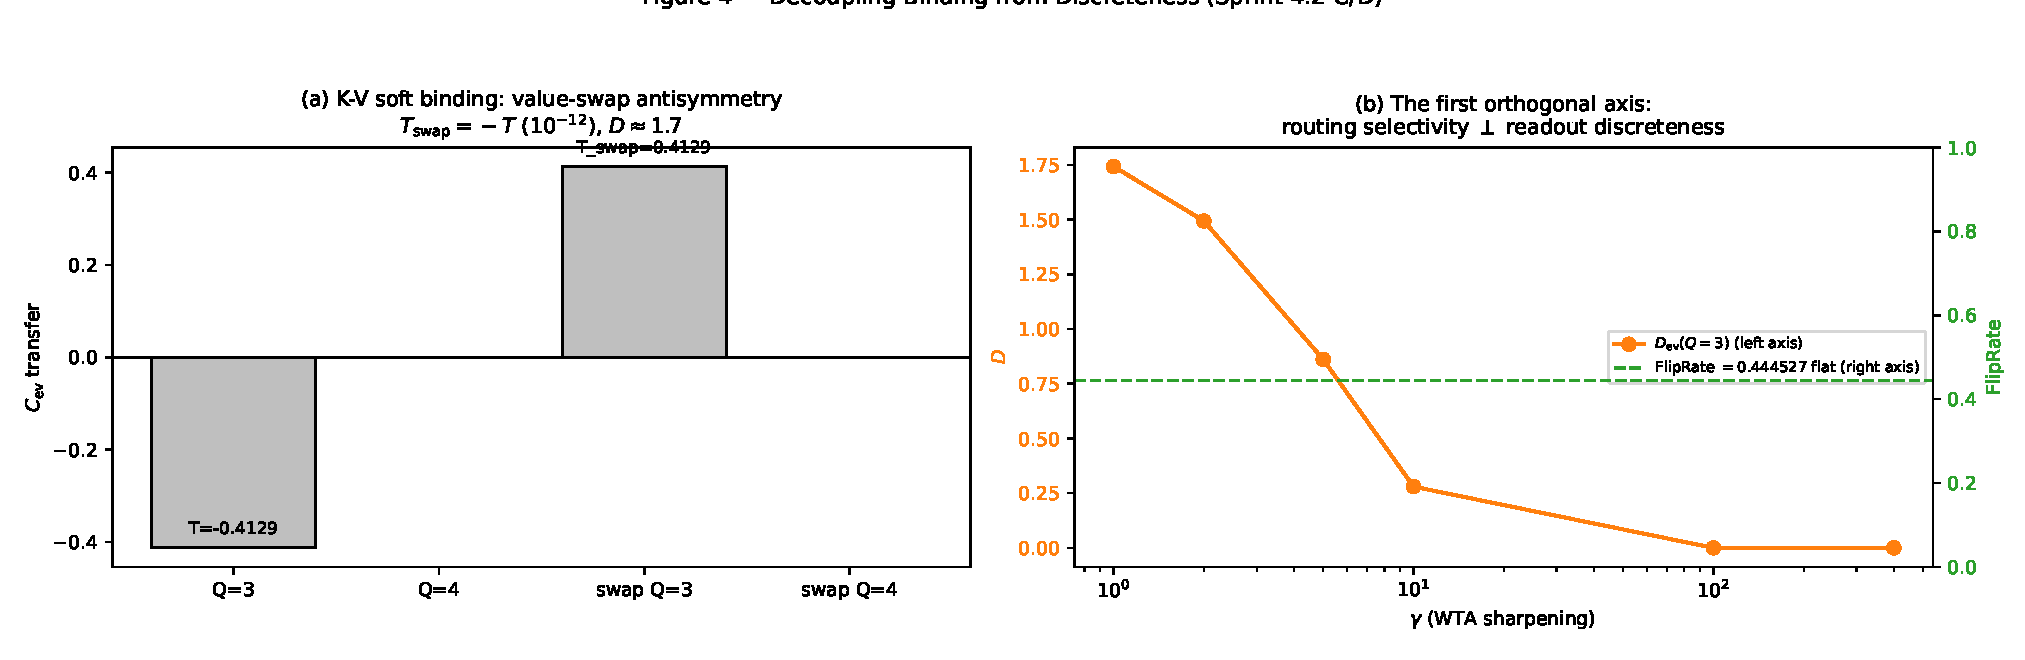
\includegraphics[width=\textwidth]{fig4_binding}
\caption{Decoupling binding from discreteness (Sprints 4.2-C/D). (a) The
soft-binding readout transfers winner-aligned value and the value-swap
counterfactual is exactly antisymmetric ($T_{\mathrm{swap}}=-T$ to
$10^{-12}$), while the softness distance stays positive. (b) The WTA
sharpening ladder: the softness collapses to zero only in the one-hot
limit, while the routing flip rate stays exactly flat ($0.444527$)---the
first orthogonal axis, routing selectivity $\perp$ readout discreteness.}
\label{fig:binding}
\end{figure}

\begin{proposition}[Argmax invariance under sharpening]
\label{prop:sharpinv}
For every $\gamma>0$,
\[
\operatorname{argmax}_i\operatorname{softmax}_i(\gamma e_i)=
\operatorname{argmax}_i e_i .
\]
Consequently all argmax-level routing statistics---winners, flip rates,
and swap antisymmetries---are invariant along the sharpening ladder, while
the readout discreteness changes from fully soft ($\gamma=1$) to fully
discrete ($\gamma=\infty$).
\end{proposition}

Proposition~\ref{prop:sharpinv} together with the measured flatness of the
flip rate formalizes the first orthogonal axis of the paper:
\emph{routing selectivity $\perp$ readout discreteness}. A model's ability
to reorder candidates and its ability to deliver a symbol are independent
organizational degrees of freedom; no amount of sharpening buys routing,
and no amount of routing buys discreteness.

\subsection{The E-I pathway crossing}
\label{sec:pathway}

The transmission audit of §6 found the E-I circuit inverting the
value-transfer direction at $\gamma=1$ ($+0.2367$; Amendment AM4). The
frozen ladder resolves that inversion: the drive transfer runs
$+0.2367\to+0.2516\to+0.0157\to-1.0541\to-3.8034\to-3.8674$, crossing zero
at the pre-registered bisection root $\gamma^*=5.098015$ where the net drive transfer
changes sign ($T_{\mathrm{drive}}=0$), thereby restoring the positive value-transfer
direction for all $\gamma > \gamma^*$, and settling at
the hard limits $A_E(\infty,3)=1.1134$, $A_E(\infty,4)=4.9809$. The
mechanism is transparent in the frozen outputs: once WTA pins the
inhibitory branch to its own winner (value $5$ at both queries), the
inhibitory term stops re-reading the increasing value channel, and the
excitatory branch's transfer ($5\to9$) re-dominates. The precise statement
carried forward is the one frozen in §6: E-I organization does not
implement binding; it \emph{reshapes the effective value-transfer pathway
after} query-conditioned routing---and WTA changes which pathway shape is
realized.

\subsection{The single-head bottleneck}
\label{sec:bottleneck}

The last frozen result of the section is a bottleneck, stated here as the
bridge to composition.

\begin{proposition}[Single-head bottleneck]
\label{prop:singlehead}
A single attention head with a scalar readout delivers, at each instant, one scalar mixture
$y = \sum_i \alpha_i v_i$ of candidate values. While a single head can evaluate symmetric
scalar pooling functions over candidates (for example, uniform weighting yielding the arithmetic
mean $\frac{1}{2}(V_A+V_B)$, which downstream scaling can map to $V_A+V_B$), its scalar output
channel cannot simultaneously deliver two distinct, independently bound operands $(V_A, V_B)$
to downstream general or non-symmetric algebra (e.g., $V_A - V_B$). At $\gamma=\infty$, the readout
collapses to a single discrete symbol $v_{\mathrm{winner}}$. Hence exact delivery of \emph{one}
bound value does not provide general two-operand composition: $\text{Exact Delivery}\not\Rightarrow
\text{Composition}$.
\end{proposition}

The identifiability audit already anticipated the trap this bottleneck
creates. With $V_A=0$, the single-winner model's composition error
vanishes ($|V_B-(0+V_B)|=0$) although its binding error does not
($E_{\mathrm{bind},A}=|V_B|>0$): the three-error joint audit of §2.5 flags
the configuration as \textsc{composition fail} and only the dual-channel
model passes the same configuration genuinely ($E_{\mathrm{bind}}=0$ and
$E_{\mathrm{comp}}=0$). This zero-value trap is retained as one of the
eight counterfactuals of §8.

\subsection{Honest notes on exactness}
\label{sec:notes7}

Two caveats are frozen with the results and repeated here. First, the
full-window softness $D_{\mathrm{full}}(3)$ is \emph{not} monotone: it
overshoots and crosses zero at $\gamma\approx1.1978$---a cancellation
artifact in which the residual value of the loser compensates the mass
lost to the silent slots, while the event-normalized softness remains
$\approx1.5$ (frozen Amendment AM5). That zero is not hard binding and is
reported as such. Second, exactness belongs to the limit: every finite
$\gamma$ is soft, so ``hard binding'' is realized here as the
$\gamma=\infty$ limit of a frozen mechanism family, not as a finite
parameter setting. Both caveats carry into the claim ledger of §10.

% ==========================================================================
% Paper 2 — Section 8: From Binding to Composition. Overcoming the
% Single-Head Bottleneck (TAN-II Sprint 4.3-A, frozen).
% ==========================================================================
\section{From Binding to Composition: Overcoming the Single-Head
Bottleneck}
\label{sec:composition}

Proposition~\ref{prop:singlehead} states the wall: one head, one symbol.
This section adds the two minimal degrees of freedom that cross it---a
second parallel channel and one two-input algebraic node (operator O5 of
§2.4)---and reports the frozen Sprint 4.3-A audits that separate binding
from composition. The central empirical statement is the second orthogonal
axis of the paper: \emph{binding fidelity $\perp$ combiner error}.

\subsection{The dual-query window}
\label{sec:dualwindow}

The frozen dual-query window is $[A,0,B,Q_1,Q_2]$ (window length $W=5$
kept), with events in the first three slots, queries in the last two, and
the shared window mean $\mu=(K_A+K_B+Q_1+Q_2)/5=2.56$ on the canonical
keys. The query pair $(Q_1,Q_2)=(4.5,5.3)$ is frozen by a
direction-targeting derivation, not by fitting: the pair is required to
rotate the two query directions $\theta_c=\omega S_c$ onto the two key
directions ($\approx44.5^{\circ}$ and $\approx62.8^{\circ}$ versus
$45^{\circ}$ and $63.4^{\circ}$), giving frozen routing margins
$m_A=+0.210631046$ and $m_B=+0.261878523$ (the pre-registration's
hand-computed values $0.2118$/$0.2637$ were four-decimal estimates; the
deviation is recorded as Amendment AM6 with the closed forms adopted and
the originals preserved). Channel $c\in\{1,2\}$ is keyed to slot $3+c$;
queries are control signals, never candidates, and carry value zero.

\subsection{The M0--M1--M2 ladder}
\label{sec:ladder8}

Three models instantiate the negative-control chain of §2.5 on the
canonical scenarios S1 $(5,9)$, S2 $(7,-2)$, S3 $(2,6)$, with operators
$f\in\{+,-\}$. The frozen error table (all values exact):

\begin{itemize}[leftmargin=*,noitemsep,topsep=1pt]
\item \emph{M0 (single winner).} Delivers exactly one operand:
$E_{\mathrm{bind},B}=0$, $E_{\mathrm{bind},A}=|V_B-V_A|>0$, and
$E_{\mathrm{comp}}=|V_A|>0$ for addition (e.g.\ $5$, $7$, $2$ on
S1/S2/S3); the zero-value trap of §7 is re-audited and caught by the
joint criterion.
\item \emph{M1 (parallel binding).} Both channels bind exactly
($E_{\mathrm{bind},A}=E_{\mathrm{bind},B}=0$), and the output is the
\emph{pair} $(\hat V_A,\hat V_B)$: composition is
\textsc{structurally undefined} because no operator connects the two
channels. The frozen non-compositional scalar projection (second-channel
readout, pre-registered as a control) fails with
$E_{\mathrm{comp}}=|V_B-f(V_A,V_B)|>0$: two correctly bound operands are
\emph{not} a composition.
\item \emph{M2 (parallel binding + one two-input combiner).} The node
$y=f(\hat C_1,\hat C_2)$ achieves $E_{\mathrm{bind},A}=E_{\mathrm{bind},B}
=E_{\mathrm{comp}}=0$ exactly on all three scenarios and both operators
($y=14,5,8$ for $+$; $-4,9,-4$ for $-$): the minimal composition node
converts parallel binding into explicit composition.
\end{itemize}

\subsection{The second orthogonal axis and the separation theorem}
\label{sec:separation}

The ensemble audit (keys i.i.d.\ $U(0.3,2.5)$, values i.i.d.\ $U(-3,3)$,
positions and orders randomized, seeds $20260904$--$06$, $N=10^4$ each)
separates the combiner's intrinsic error from the propagated binding
error. Frozen benchmarks (deterministic $2001^2$ quadrature) establish: per-channel
routing rates $r_A=r_B=0.499750$, both-routed probability $P_{\mathrm{both}}=0.220725$ ($22.07\%$),
and unconditional composition errors $E[E_{\mathrm{comp}}^+]=1.116099621$,
$E[E_{\mathrm{comp}}^-]=2.000999500$. The 30,000-history Monte Carlo simulation (seeds $20260904$--$06$,
$N=10^4$ each) yields empirical pooled means of $E[E_{\mathrm{comp}}^+]=1.107671595$
(seed-level: $1.120449 / 1.074606 / 1.127960$) and $E[E_{\mathrm{comp}}^-]=1.975892767$
(seed-level: $1.989288 / 1.959625 / 1.978765$), matching quadrature benchmarks within sampling variance.
The empirical both-routed subset spans $6{,}608 / 30{,}000$ trials ($22.0267\% \approx 22.03\%$;
$2{,}188 / 2{,}258 / 2{,}162$ per seed).

\begin{figure}[t]
\centering
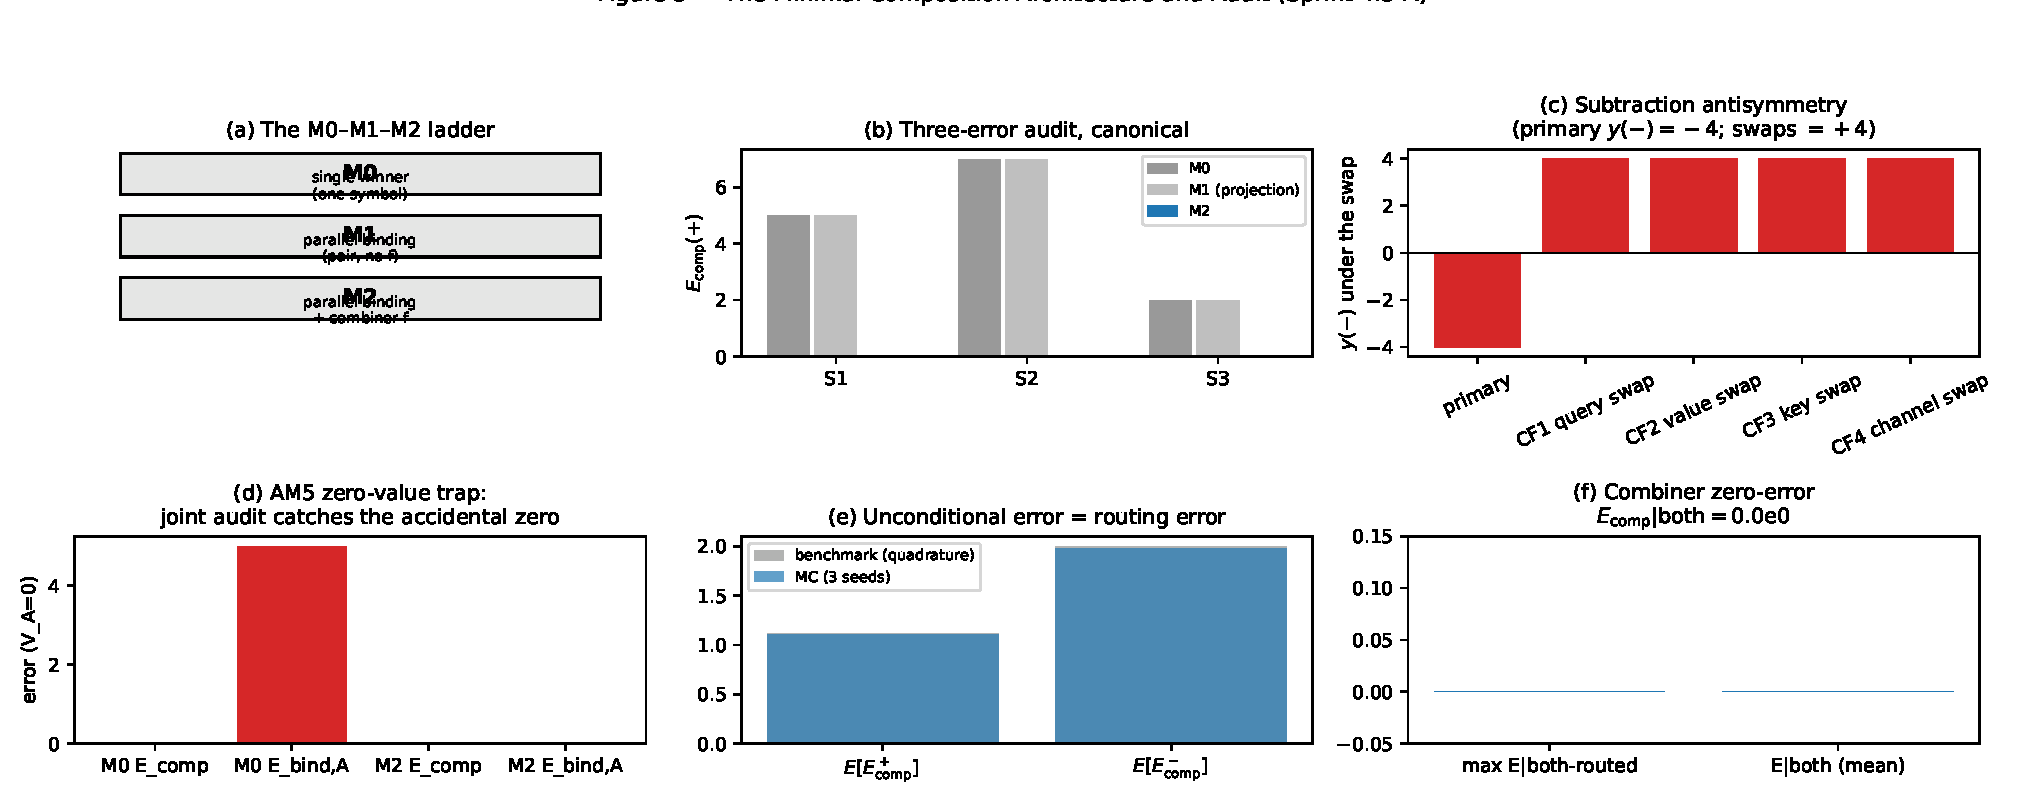
\includegraphics[width=0.70\textwidth]{fig5_composition}
\caption{The minimal composition architecture and audit (Sprint 4.3-A).
(a) The M0--M1--M2 ladder: one winner, two channels, two channels plus one
two-input combiner. (b) The canonical three-error audit across scenarios
S1/S2/S3: only M2 reaches zero composition error. (c) Subtraction
antisymmetry across the four swap counterfactuals. (d) The zero-value trap:
M0's accidental composition zero is caught by the binding error. (e)
Unconditional composition error equals the routing-error benchmark.
(f) Conditioned on correct binding, the combiner error is exactly
$0.0\mathrm{e}0$.}
\label{fig:composition}
\end{figure}

\begin{proposition}[Binding--combiner error separation]
\label{prop:separation}
Given exact operand delivery ($\hat C_c=V_c$ for both channels), the
frozen combiner computes $f$ exactly, so
$E_{\mathrm{comp}}\mid\text{both-routed}=0$. Empirically the maximum over
$3\times10^4$ histories is exactly $0.0\mathrm{e}0$: the combiner adds
zero error, and every unit of unconditional composition error is the
propagation of an upstream routing error
(\emph{routing error $\to$ wrong operand $\to$ composition error}).
\end{proposition}

Proposition~\ref{prop:separation} is the second orthogonal axis:
\emph{binding fidelity $\perp$ combiner error}. Composition capability and
binding fidelity are independent organizational quantities in this family;
the combiner's quality is a property of the algebraic node, the
unconditional error a property of the geometry upstream of it.

\enlargethispage{2\baselineskip}
\subsection{The eight counterfactuals}
\label{sec:cf8}

All eight frozen counterfactuals passed ($\PassFailInconclusive{}$
verdicts, deterministic):

\begin{enumerate}[leftmargin=*,noitemsep,topsep=1pt]
\item \emph{Query swap.} $(Q_1,Q_2)\to(Q_2,Q_1)$: addition invariant,
subtraction exactly antisymmetric ($y\to-y$).
\item \emph{Value swap.} $(K_A,V_B),(K_B,V_A)$: addition invariant
(correct commutative behavior---scored against the channel-level swap
$(9,5)$ as the pairing check, never as a false negative), subtraction
antisymmetric.
\item \emph{Key swap} (keys exchanged, value pairing kept): addition
invariant, subtraction antisymmetric.
\item \emph{Channel-output swap} at the combiner inputs: addition
invariant, subtraction antisymmetric.
\item \emph{AM5 zero-value trap.} $V_A=0$: M0's composition error
vanishes while its binding error does not---caught by the joint audit;
M2 passes genuinely. \textsc{pass}.
\item \emph{Binding-preserving counterfactual.} Value shift
$(5,9)\to(7,11)$: all three errors stay zero and $y=18$; the legacy
single-query controls ($3.0\to A$, $4.0\to B$) reproduce the frozen 4.2-D
routing. \textsc{pass}.
\item \emph{Binding-breaking counterfactual.} Legacy queries $(3.0,4.0)$
in the dual window mis-route channel 2:
$E_{\mathrm{bind},B}=4$ and $E_{\mathrm{comp}}=4$---the causal chain
\emph{routing $\to$ binding $\to$ operand delivery $\to$ composition} is
demonstrated by its failure mode. \textsc{pass}.
\item \emph{Composition-sensitive relational counterfactual.} Across the
three scenarios the output equals $f$ exactly and subtraction
distinguishes the relations ($-4,9,-4$). \textsc{pass}.
\end{enumerate}

Position randomization (six orderings) is bitwise-invariant ($10^{-12}$),
query leakage is excluded ($Q\cap V=\varnothing$; queries never
candidates; query slots carry value zero), and the query-order swap pass
over the whole ensemble preserves addition and antisymmetrizes subtraction
history by history.

\enlargethispage{2.5\baselineskip}
\subsection{The dynamical carrier and spiking readout audit: Phase P1-B}
\label{sec:carrier_audit}

The static algebraic node of \S\ref{sec:ladder8}--\ref{sec:separation} combines
retrieved operand values ($y = C_1 \pm C_2$) once delivered. However, in an online
neural substrate, operands must be continuously maintained and routed through the
internal dynamical state of the neuron, and transmitted across discrete spiking channels
to downstream integrators. Phase~P1-B subjected this continuous dynamical carrier to a pre-registered
confirmatory audit under Protocol~V2.6.

\paragraph{Continuous carrier dynamics and subthreshold state collisions.}
The continuous-time Temporal Attention Neuron carrier evolves as a three-variable ODE
$\mathbf{z}(t) = [u(t), A(t), r(t)]^T$:
\begin{equation}
\tau_u \dot{u}(t) = -u(t) + I(t), \quad
\tau_A \dot{A}(t) = -A(t) + \sigma_A(u(t)), \quad
\tau_r \dot{r}(t) = -r(t) + A(t) \cdot u(t),
\label{eq:p1b_carrier}
\end{equation}
where $I(t)$ is the incoming current pulse sequence, $\sigma_A(\cdot)$ is the
attention activation with threshold $\theta_A$, and $r(t)$ is the surprise-weighted
carrier. At query arrival time $t_Q$, an affine decoder maps the state to delivered operand values:
$\hat{v}_c = g_{\text{dec}} r(t_Q) + b_{\text{dec}}$ ($g_{\text{dec}} = 0.132630817$, $b_{\text{dec}} = -0.026816484$).
Pre-registered fixture G1.5 proved an analytical subthreshold collision theorem: for any interval where $u(t) < \theta_A$,
$\sigma_A(u(t)) \equiv 0$, forcing unmodulated exponential decay $\dot{A} = -A/\tau_A$ and $\dot{r} = -r/\tau_r$.
Consequently, distinct temporal history sequences that differ only during subthreshold periods collapse to analytically identical state vectors $\mathbf{z}(t_Q)$ (residual $< 10^{-10}$), erasing subthreshold events prior to query arrival.

\paragraph{Confirmatory evaluation: floor-limited comparison and unestablished redundancy.}
The confirmatory audit spanned 4,000 unique histories across 3 post-sequence silence
delays ($\Delta t_{\text{silence}} \in \{0, 5, 10\}\,\text{ms}$) and 8 model variants,
totaling 96,000 model-episodes (192,000 role queries). Protocol~V2.6 \S7.3 registered
prerequisite joint delivery accuracy floors ($E_{\text{bind}} \le 0.05$ on both channels)
of $0.80$ for $N=2$ and $0.40$ for $N=3$. The baseline dynamical carrier M1 (evolving from $A(0)=0$) achieved joint delivery accuracy of only $0.0290$ ($58/2{,}000$) for $N=2$ across all delays, and $0.0275$--$0.0280$ ($55$--$56/2{,}000$) for $N=3$. Failing the prerequisite in every cell, all conditions are classified as \texttt{FLOOR\_LIMITED\_COMPARISON}. Two One-Sided Tests (TOST, margin $\pm 0.05$) showed that M1 and the memory-lesioned constant-gate control M2a ($A(t) \equiv A_0 = 0.061886726$) are statistically equivalent within tight $90\%$ confidence intervals ($N=2$: $[-0.001515, 0.001515]$; $N=3$: $[-0.002978, 0.000841]$ at $0\,\text{ms}$, $[-0.002262, 0.001186]$ at $5, 10\,\text{ms}$). However, because both models reside near zero accuracy, this statistical equivalence is an artifact of mutual baseline failure, \emph{not} evidence that temporal gating dynamics are redundant (\texttt{redundancy\_inferred = False}).

\paragraph{Spiking channel limitation.}
To evaluate neural transmission to downstream algebra, carrier states were converted into spike trains via single-unit leaky integrate-and-fire (LIF) decoders under rate (M4\_Count) and first-spike latency (M4\_Latency) codes. Under the registered limitation criterion $E_{\text{comp}} \ge 0.05$, both decoders exhibited severe breakdown across all cells ($E_{\text{comp}} \in [2.21, 2.57]$). Delay-pooled $95\%$ bootstrap confidence intervals were: $N=2$: M4\_Count $[2.393533, 2.502027]$, M4\_Latency $[2.243582, 2.332606]$; $N=3$: M4\_Count $[2.473506, 2.571918]$, M4\_Latency $[2.212398, 2.296450]$. High episode-level abstention rates ($82.1\%$--$83.0\%$; single-query silence $57.15\%$--$58.60\%$) confirm that single-unit spiking decoders cannot reliably transmit continuous-carrier operands, certifying \texttt{DEMONSTRATED\_CHANNEL\_LIMITATION}.

\subsection{Scope of the rung}
\label{sec:scope8}

The established statement is a sufficiency result inside the frozen mechanism family: \emph{parallel binding plus one minimal two-input combiner suffices for identifiable composition, with zero combiner error conditioned on correct binding}. Crucially, this zero composition error is strictly conditional: across the full ensemble of $30{,}000$ histories ($3\times10^4$), the both-routed subset comprises $6{,}608$ histories ($22.03\%$, matching the $22.07\%$ unguided benchmark), with unconditioned pooled errors of $1.108$ ($+$) and $1.976$ ($-$) reflecting upstream routing.

Furthermore, the consensus determination certified under Protocol~V2.6 establishes that M1 fails the baseline delivery prerequisite across all conditions ($2.75\%$--$2.90\%$ joint accuracy), rendering comparisons floor-limited and leaving memory redundancy unestablished, while tested spiking readouts demonstrate channel limitation for single-unit point-process decoders ($E_{\text{comp}} > 2.2$, $82\%$ abstention). These findings establish \emph{model-specific insufficiency} for the continuous ODE carrier and frozen linear readout, not a universal biological impossibility result or a proven requirement for population coding. Internal composition dynamics (Hypothesis~H3), multi-operand composition, and learned operators remain formally deferred.

% ==========================================================================
% Paper 2 — Section 9: The Unified Mechanistic Ladder & General Discussion.
% ==========================================================================
\section{The Unified Mechanistic Ladder and General Discussion}
\label{sec:ladder}

The eight preceding sections assembled one rung at a time. This section
assembles the whole: the master table of the ladder (§9.1), the two
orthogonal axes as the paper's conceptual residue (§9.2), the biological
reading of each organizational degree of freedom---explicitly as a mapping
of \emph{degrees of freedom}, not as an equivalence claim (§9.3)---and the
general discussion (§9.4).

\subsection{The master table}
\label{sec:master}

Table~\ref{tab:ladder} compresses the ladder. Each row names the single
added organizational degree of freedom, the primitive it certifies, the
boundary wall the frozen audits located at that rung, and the decisive
experiment. Two reading rules apply. First, the walls are results, not
footnotes: every $\not\Rightarrow$ in the table is backed by an exact
number (a zero flip rate, a positive softness distance, a positive binding
error). Second, the ladder is constructive in the tested family and
\emph{sufficient}, not necessary: the paper claims that these degrees of
freedom suffice here, never that they are the only possible ones.

\begin{table}[t]
\centering
\small
\setlength{\tabcolsep}{4pt}
\begin{tabular}{@{}p{1.4cm}p{2.7cm}p{3.0cm}p{3.2cm}p{3.2cm}@{}}
\toprule
Rung & Added DOF & Certified primitive & Boundary wall (frozen) &
Decisive audit \\
\midrule
L0 & (frozen baseline) & Memory & --- & Collision $K$: B1 $0.5$ exact vs B4
$2.047\times10^{4}$; post-reset $0$ vs $32.2\%$ \\
L1 & surprise-gated window & Saliency weighting & Order-locked:
$\operatorname{argmax}$ query-invariant & FlipRate $0.000$; Probe-2
\textsc{terminated} / \textsc{audit\_failed} \\
L2 & (measurement rung) & Geometric reorganization & Effective rank
$\neq$ intrinsic dimension; no selectivity & $d_D$ $2.089$ vs $1.484$;
shared-frame B4 $\not>$ B1 \\
L3 & O1 opponent competition & Nonmonotone selective tuning &
$\text{Competition}\not\Rightarrow\text{Routing}$ & Theorem 4.1; C1 peak
$x^*=1.00$; six layouts FlipRate $0.000$ \\
L4 & O2 vector Q-K & Content routing &
representation-family-dependent & Flip law $\theta/\pi$ (132/132);
$+0.2587\to-0.1559$; $0.4425$ vs $0.4445$; AM2 \\
L5 & O3 K-V + O4 WTA & Binding; exact delivery &
softmax mixing barrier; exactness only in the discrete limit &
$T_{\mathrm{swap}}=-T$ ($10^{-12}$); $\gamma$ ladder $D\to0$; flat
flip rate $0.4445$ \\
L6 & O5 parallel channels + combiner & Composition &
$\text{Binding}\not\Rightarrow\text{Composition}$; unconditional error
$=$ routing error & M0/M1/M2 chain; 8 counterfactuals;
$E_{\mathrm{comp}}|\text{both-routed}\equiv0$ \\
\bottomrule
\end{tabular}
\caption{The unified mechanistic ladder. Each row is one frozen sprint;
the walls are the paper's negative results, each with its exact
statistic.}
\label{tab:ladder}
\end{table}

\begin{figure}[t]
\centering
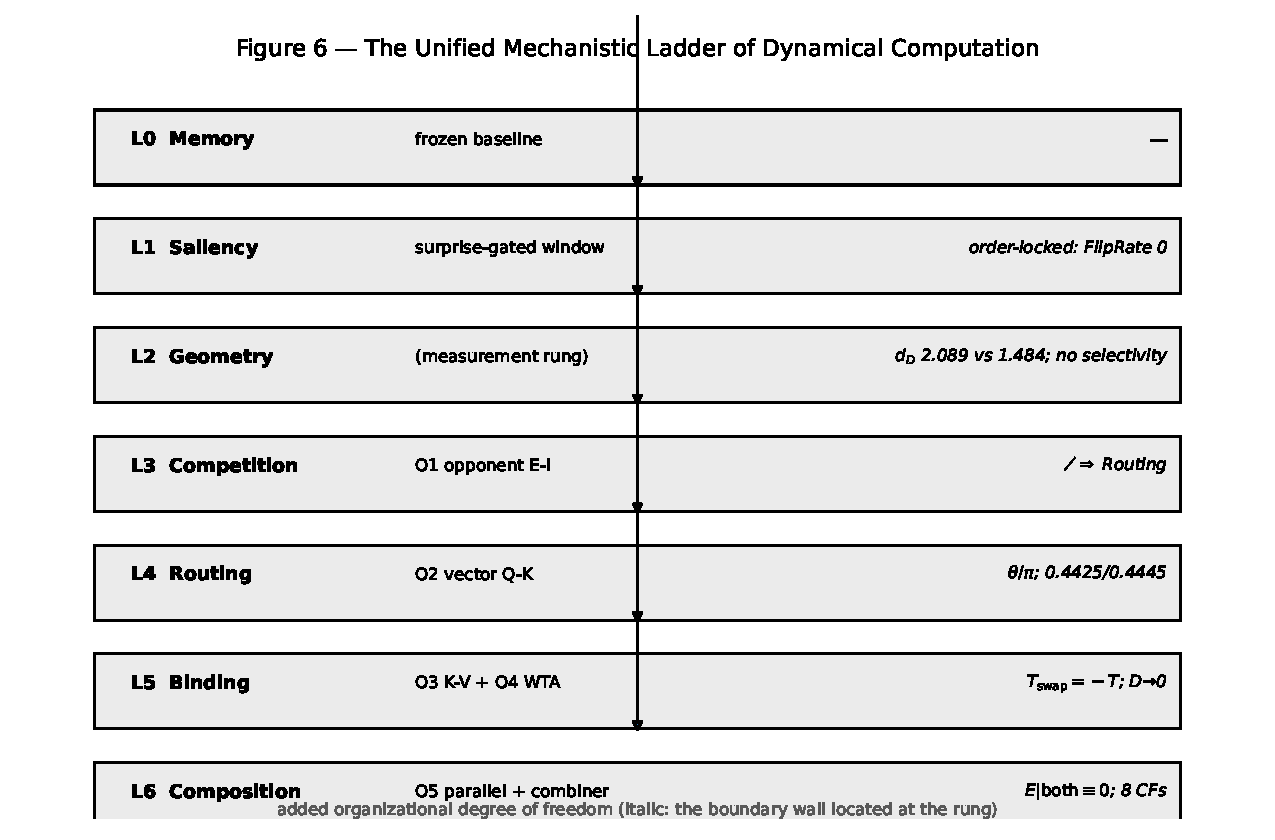
\includegraphics[width=0.72\textwidth]{fig6_ladder}
\caption{The unified mechanistic ladder of dynamical computation. Each
rung names the single added organizational degree of freedom and, in
italics, the boundary wall located at that rung by the frozen audits.}
\label{fig:ladder}
\end{figure}

\subsection{The two orthogonal axes}
\label{sec:axes}

The ladder's most transferable residue is a pair of orthogonal axes that
the audits forced into view.

\emph{Axis 1: routing selectivity $\perp$ readout discreteness} (§7).
Sharpening from soft mixing to one-hot selection changes \emph{how} a
winner is delivered, never \emph{which} winner is selected: the flip rate
is exactly flat ($0.444527$) across the entire WTA ladder, while the
softness distance collapses from $1.74$ to $0$. A model's reordering
capacity and its symbol-delivery capacity are independent purchases.

\emph{Axis 2: binding fidelity $\perp$ combiner error} (§8). The combiner
contributes exactly zero error conditioned on correct operand delivery
(measured maximum $0.0\mathrm{e}0$ over $3\times10^4$ histories), while
the unconditional composition error is entirely the propagation of
upstream routing errors. A model's ability to compose and its ability to
bind are independent purchases, separated by the operand-delivery step.

Together the axes state the paper's architectural thesis in measurable
form: capability in this substrate is organized along \emph{named,
independent} degrees of freedom, so that no single scalar (accuracy, loss,
rank, sharpness) can stand in for any of them---each rung owns its own
audit, and the audits are the ladder.

\enlargethispage{2\baselineskip}
\subsection{Biological reading: degrees of freedom, not equivalences}
\label{sec:bio}

The paper's organizational degrees of freedom have natural biological
counterparts, and the blueprint fixes the mapping to be read strictly as
an analogy between \emph{kinds of organization}, never as a claim that the
tested neuron is any particular biological circuit.

\begin{itemize}[leftmargin=*,noitemsep,topsep=1pt]
\item \emph{Opponent competition (L3).} The E-I microcircuit is the
canonical organizational motif of cortical columns
\citep{mountcastle1997}, where fast-spiking parvalbumin-positive
interneurons provide the subtractive inhibition whose functional
signature---nonmonotone, band-pass selectivity---Theorem 4.1 derives from
two inequalities alone \citep{amari1977}.
\item \emph{The two-dimensional query direction (L4).} A minimal
continuous direction space over candidate content is what oscillatory
phase (a circular variable) provides to relational codes
\citep{singer1999}; the paper's content is not that phase \emph{is}
$\mathbb{R}^2$, but that a connected one-dimensional query manifold is the
minimal geometry in which query-conditioned reordering becomes continuous.
\item \emph{Parallel binding channels (L5--L6).} Independent nonlinear
channels converging on a common readout are the organizational signature
of dendritic computation: apical and basal compartments of pyramidal
neurons integrate separate streams before somatic output
\citep{london2005,poirazi2003}. The paper's dual-channel-plus-combiner
architecture is the minimal abstraction of exactly that arrangement, and
the axon initial segment's threshold integration is the natural candidate
for the two-input algebraic node.
\end{itemize}

The caution inherited from the frozen discipline: these are candidate
physical realizations of non-factorizable organization, not established
identities, and none of the tested numbers transfers to biology by
construction (§8.6).

\subsection{General discussion}
\label{sec:discussion}

\emph{More dynamics does not imply more computational primitives.} The
temporal memory window $W=5$ was held strictly constant throughout the ladder:
each rung does not enlarge temporal buffer capacity, but systematically introduces
distinct \emph{organizational degrees of freedom}---a second sign of coupling
(E-I opponent units), a second query dimension ($S^1$ rotation), a split between
keys and values, a sharp selection map, a second channel, and one algebraic
combiner. These additions reflect how attention and memory structures function
as fast-weight programming and energy-based associative retrieval
\citep{schlag2021,ramsauer2020}. Every rung's effect is certified by a
counterfactual that the previous rung fails. Nonlinear dynamics is
the stage on which computation happens; the primitives are the topology
erected on it.

Three questions delimit the honest reach of the work. First,
\emph{necessity}: the paper establishes sufficiency chains inside one
frozen family; it does not rule out other mechanisms that route, bind, or
compose. Second, \emph{generality}: every boundary wall is certified at
frozen parameters, frozen queries, and two to four candidates; scaling
audits (more distractors, nested operators, learned embeddings) are
explicitly out of scope and listed in §10. Third, \emph{composition's
open end}: the combiner tested is a single two-input algebraic node; what
minimal organization suffices for multi-operand or nested composition is
the natural next rung, and the paper leaves it unclaimed.

What the paper does claim, and defends with exact numbers, is a boundary
map: for each rung from memory to composition, the minimal organizational
condition under which the primitive appears in this substrate, and the
exact statistic at which the previous rung stops. That map, not any single
model, is the intended contribution.

\enlargethispage{3\baselineskip}
\section{Claim Ledger and Reproducibility Statement}
\label{sec:ledger}

This closing section grades every claim of the paper (Table~\ref{tab:claims})
and states the reproducibility conditions under which every number in the
preceding sections can be regenerated.

\subsection{The claim ledger}
\label{sec:claims}

Levels: \textsc{established} (deterministic / analytical / numerical
evidence, with exact statistics), \textsc{supported} (statistical support
without a closed-form theorem), \textsc{rejected} (explicitly negated by
experiment), \textsc{unknown} (insufficient evidence in this programme).
\clearpage

\begin{table}[p]
\centering
\footnotesize
\renewcommand{\arraystretch}{0.88}
\setlength{\tabcolsep}{3.2pt}
\begin{tabular}{@{}c>{\raggedright\arraybackslash}p{3.8cm}>{\raggedright\arraybackslash}p{2.2cm}>{\raggedright\arraybackslash}p{4.6cm}>{\raggedright\arraybackslash}p{3.0cm}@{}}
\toprule
\# & Claim & Level & Frozen evidence & Anti-false-positive guard \\
\midrule
C1 & The scalar TAN has memory: its state is not Markov-sufficient &
\textsc{established} & $N=160{,}000$; $K$ mean: $0.5$/$4.47\mathrm{e}3$/$1.235\mathrm{e}4$/$2.047\mathrm{e}4$; median: $0.5$/$896$/$1.37\mathrm{e}3$/$2.95\mathrm{e}3$; post-reset $0$/$0.6$/$33.1$/$32.2\%$
& gate-closed collapse to $0.5$; resync $n=843$ \\
C2 & Positive-scalar saliency is order-locked (Theorem 5.1) &
\textsc{established} & FlipRate $0.000$; Probe-2 \textsc{terminated}/\textsc{audit\_failed} & domain-conditional statement (AM1) \\
C3 & Attention reorganizes event-locked geometry without adding selectivity &
\textsc{established} & $d_D$ $2.089$ vs $1.484$; $\Delta\log\mathrm{Tr}=1.355$ nats; B4 $\not>$ B1 shared-frame & effective rank $\neq$ intrinsic dimension \\
C4 & Nonmonotone tuning is opponent-structural; attention is gain / operating-range modulation &
\textsc{established} & Theorem 4.1; C1 peak $x^*=1.00$ ($h_E=0.200$); C2--C4 no strict maxima; predictions $4/4$ & C1 has zero attention (necessity counterexample) \\
C5 & Competition does not route &
\textsc{established} & six layouts $\times$ two variants FlipRate $0.000$; query-sensitive magnitudes only & kernel-before-dynamics argument \\
C6 & $d=2$ is minimal for continuous query direction under dot-product; flip law $\theta/\pi$ &
\textsc{established} & 132/132 isotropic conditions (140 checks total); $F_d=\tfrac12$ across $d=2,3,4,8$; ordering ladder $1/2/M(M-1)/M!$ & $F_d$ retained as negative control; dimension controls \\
C7 & The running neuron realizes counterfactual routing &
\textsc{established} & margins $+0.2587\to-0.1559$; $Q^*=3.7071$; ensemble $0.4425$ vs $0.4445$ & probe-below-winner; $\omega$-sweep structure; AM2 normalization \\
C8 & Key--value decoupling yields soft, pairing-sensitive binding &
\textsc{established} & $T=-0.4129$; $T_{\mathrm{swap}}=-T$ ($10^{-12}$); $D=1.74$/$1.84$ & value-swap antisymmetry; baselines ($0.0844$ sharpening drift) \\
C9 & The WTA limit delivers exactly; routing $\perp$ discreteness &
\textsc{established} & $\gamma$ ladder: $D\to0$ only at $\infty$; flip rate flat $0.444527$; E-I root $\gamma^*=5.098015$ & finite-$\gamma$ positivity; AM5 cancellation zero flagged \\
C10 & Exact delivery does not imply composition (single-head bottleneck) &
\textsc{established} & M0 $E_{\mathrm{comp}}=|V_A|>0$; $V_A=0$ trap caught by joint audit & three-error joint audit \\
C11 & Parallel binding plus one combiner composes; binding $\perp$ combiner error &
\textsc{established} & M2 errors $0$ (S1--S3, $+$/$-$); both-routed cov.\ $22.03\%$ ($22.07\%$ bench), $E_{\mathrm{comp}}|\text{both}\equiv0$; bench $1.116/2.001$, MC $1.108/1.976$; 8 CFs pass & separation test; swap suite; M1 structurally undefined \\
C12 & Biological readings (columns, phase, dendritic subunits) are organizational analogies &
\textsc{supported} (as mappings) & qualitative correspondence only & explicitly denied equivalence (rejected if read as identity) \\
C13 & 1D metric compatibility is sufficient for content addressing; 2D rotation not necessary &
\textsc{established} & 60,000 trials (420,000 evals); C1/C2 acc $100.00\%$; metric $\equiv$ 2D argmax; signed scalar $0/6{,}705$ on intermediate key & G1.1--G1.4 suites; chance derivation ($16.67\%$); leakage audit \\
C14 & Continuous dynamical carrier \& spiking readout audit (Phase P1-B) &
\textsc{bounded / insufficient} & 96,000 episodes (192,000 queries); 6/6 cells at mutual floor (M1 joint delivery $2.75\%$--$2.90\% < 80\%/40\%$); TOST 90\% CIs bounded; spiking $E_{\mathrm{comp}}\in[2.21, 2.57]$; abstention $82.1\%$--$83.0\%$ & pre-registered prerequisite floor rule; TOST equivalence bounds; G1.5 subthreshold collision theorem (res $<10^{-10}$); H3 deferred; model-specific insufficiency \\
\bottomrule
\end{tabular}
\caption{Master claim ledger. Levels follow \S2.5's frozen discipline; every \textsc{established} row carries its exact statistic and the audit that protects it.}
\label{tab:claims}
\end{table}
\clearpage

\subsection{Reproducibility statement}
\label{sec:repro}
\enlargethispage{3\baselineskip}

\emph{Archives.} All quantitative statements of this paper are read from
the frozen archives: the TAN-I dossier, collision and geometry logs, the
Probe-1 amended audit, the Probe-2 identifiability archive, the TAN-II
sprint registry 4.1--4.3-A (pre-registrations, amendments AM1--AM6,
deterministic scripts, and machine-readable summaries), the Phase~P1-A
address identifiability archive (60,000 trials, 420,000 evaluations),
and the Phase~P1-B dynamical carrier audit dossier (Protocol~V2.6
\texttt{07D58A2D\dots}, 12-fixture G1 suite, 96,000 episodes, confirmatory manifest
\texttt{08EC79B9\dots}). No frozen file was modified for this manuscript; the manuscript's numbers were extracted, not recomputed.

\emph{Determinism.} Every experiment is deterministic under the fixed
seeds $20260904$, $20260905$, $20260906$ ($N=10^4$ per seed where Monte
Carlo applies) with no random-state drift; analytic benchmarks are
deterministic $2001^2$ quadratures of the frozen model; structural
identities are asserted at $10^{-12}$; the environment is Python 3.12
with NumPy/SciPy/Matplotlib only. Each sprint script records its own
SHA-256 in its output summary.

\emph{Pre-registration and amendments.} Every rung's predictions were
frozen before its run. Six discrepancies were found---AM1 (the E4(iii)
closed-form value), AM2 (the unnormalized-control expectation), AM3
(corrected fixed-point constants), AM4 (the E-I drive-transfer value),
AM5 (the readout-softness monotonicity and its cancellation zero), AM6
(the canonical routing margins)---and all six were handled by the frozen
protocol: stop, independently recompute, record the cause in a dated
amendment that preserves the original prediction verbatim, then continue.
None altered a model, query, seed, or threshold; the originals remain in
the archive.

\emph{Open problems (explicitly not claimed).} General symbolic
reasoning; multi-distractor ($N>2$) generalization; necessity (versus
sufficiency) of the tested mechanisms; nested or multi-operand
composition; internal composition dynamics (Hypothesis~H3, formally deferred);
learned representations; and any biological equivalence (C12). These are the
next rungs of the programme, and the paper's boundary map is offered as the
instrument for auditing them.


\bibliographystyle{plainnat}
\bibliography{references}

\end{document}
